\documentclass[twoside]{book}

% Packages required by doxygen
\usepackage{fixltx2e}
\usepackage{calc}
\usepackage{doxygen}
\usepackage[export]{adjustbox} % also loads graphicx
\usepackage{graphicx}
\usepackage[utf8]{inputenc}
\usepackage{makeidx}
\usepackage{multicol}
\usepackage{multirow}
\PassOptionsToPackage{warn}{textcomp}
\usepackage{textcomp}
\usepackage[nointegrals]{wasysym}
\usepackage[table]{xcolor}

% Font selection
\usepackage[T1]{fontenc}
\usepackage[scaled=.90]{helvet}
\usepackage{courier}
\usepackage{amssymb}
\usepackage{sectsty}
\renewcommand{\familydefault}{\sfdefault}
\allsectionsfont{%
  \fontseries{bc}\selectfont%
  \color{darkgray}%
}
\renewcommand{\DoxyLabelFont}{%
  \fontseries{bc}\selectfont%
  \color{darkgray}%
}
\newcommand{\+}{\discretionary{\mbox{\scriptsize$\hookleftarrow$}}{}{}}

% Page & text layout
\usepackage{geometry}
\geometry{%
  a4paper,%
  top=2.5cm,%
  bottom=2.5cm,%
  left=2.5cm,%
  right=2.5cm%
}
\tolerance=750
\hfuzz=15pt
\hbadness=750
\setlength{\emergencystretch}{15pt}
\setlength{\parindent}{0cm}
\setlength{\parskip}{3ex plus 2ex minus 2ex}
\makeatletter
\renewcommand{\paragraph}{%
  \@startsection{paragraph}{4}{0ex}{-1.0ex}{1.0ex}{%
    \normalfont\normalsize\bfseries\SS@parafont%
  }%
}
\renewcommand{\subparagraph}{%
  \@startsection{subparagraph}{5}{0ex}{-1.0ex}{1.0ex}{%
    \normalfont\normalsize\bfseries\SS@subparafont%
  }%
}
\makeatother

% Headers & footers
\usepackage{fancyhdr}
\pagestyle{fancyplain}
\fancyhead[LE]{\fancyplain{}{\bfseries\thepage}}
\fancyhead[CE]{\fancyplain{}{}}
\fancyhead[RE]{\fancyplain{}{\bfseries\leftmark}}
\fancyhead[LO]{\fancyplain{}{\bfseries\rightmark}}
\fancyhead[CO]{\fancyplain{}{}}
\fancyhead[RO]{\fancyplain{}{\bfseries\thepage}}
\fancyfoot[LE]{\fancyplain{}{}}
\fancyfoot[CE]{\fancyplain{}{}}
\fancyfoot[RE]{\fancyplain{}{\bfseries\scriptsize Generated by Doxygen }}
\fancyfoot[LO]{\fancyplain{}{\bfseries\scriptsize Generated by Doxygen }}
\fancyfoot[CO]{\fancyplain{}{}}
\fancyfoot[RO]{\fancyplain{}{}}
\renewcommand{\footrulewidth}{0.4pt}
\renewcommand{\chaptermark}[1]{%
  \markboth{#1}{}%
}
\renewcommand{\sectionmark}[1]{%
  \markright{\thesection\ #1}%
}

% Indices & bibliography
\usepackage{natbib}
\usepackage[titles]{tocloft}
\setcounter{tocdepth}{3}
\setcounter{secnumdepth}{5}
\makeindex

% Hyperlinks (required, but should be loaded last)
\usepackage{ifpdf}
\ifpdf
  \usepackage[pdftex,pagebackref=true]{hyperref}
\else
  \usepackage[ps2pdf,pagebackref=true]{hyperref}
\fi
\hypersetup{%
  colorlinks=true,%
  linkcolor=blue,%
  citecolor=blue,%
  unicode%
}

% Custom commands
\newcommand{\clearemptydoublepage}{%
  \newpage{\pagestyle{empty}\cleardoublepage}%
}

\usepackage{caption}
\captionsetup{labelsep=space,justification=centering,font={bf},singlelinecheck=off,skip=4pt,position=top}

%===== C O N T E N T S =====

\begin{document}

% Titlepage & ToC
\hypersetup{pageanchor=false,
             bookmarksnumbered=true,
             pdfencoding=unicode
            }
\pagenumbering{roman}
\begin{titlepage}
\vspace*{7cm}
\begin{center}%
{\Large Estructuras de Datos Lineales }\\
\vspace*{1cm}
{\large Generated by Doxygen 1.8.11}\\
\end{center}
\end{titlepage}
\clearemptydoublepage
\tableofcontents
\clearemptydoublepage
\pagenumbering{arabic}
\hypersetup{pageanchor=true}

%--- Begin generated contents ---
\chapter{Hierarchical Index}
\section{Class Hierarchy}
This inheritance list is sorted roughly, but not completely, alphabetically\+:\begin{DoxyCompactList}
\item \contentsline{section}{Animal}{\pageref{classAnimal}}{}
\begin{DoxyCompactList}
\item \contentsline{section}{Lobo}{\pageref{classLobo}}{}
\item \contentsline{section}{Oveja}{\pageref{classOveja}}{}
\item \contentsline{section}{Raton}{\pageref{classRaton}}{}
\item \contentsline{section}{Zorro}{\pageref{classZorro}}{}
\end{DoxyCompactList}
\item \contentsline{section}{Celda}{\pageref{classCelda}}{}
\item \contentsline{section}{Controlador}{\pageref{classControlador}}{}
\end{DoxyCompactList}

\chapter{Data Structure Index}
\section{Data Structures}
Here are the data structures with brief descriptions\+:\begin{DoxyCompactList}
\item\contentsline{section}{\hyperlink{classBPlusTree}{B\+Plus\+Tree$<$ Data $>$} }{\pageref{classBPlusTree}}{}
\item\contentsline{section}{\hyperlink{classLeaf}{Leaf$<$ Data $>$} }{\pageref{classLeaf}}{}
\item\contentsline{section}{\hyperlink{classNode}{Node$<$ Data $>$} }{\pageref{classNode}}{}
\end{DoxyCompactList}

\chapter{File Index}
\section{File List}
Here is a list of all files with brief descriptions\+:\begin{DoxyCompactList}
\item\contentsline{section}{\hyperlink{BPlusTree_8h}{B\+Plus\+Tree.\+h} }{\pageref{BPlusTree_8h}}{}
\item\contentsline{section}{\hyperlink{Leaf_8h}{Leaf.\+h} }{\pageref{Leaf_8h}}{}
\item\contentsline{section}{\hyperlink{main_8cpp}{main.\+cpp} }{\pageref{main_8cpp}}{}
\item\contentsline{section}{\hyperlink{Node_8h}{Node.\+h} \\*Clase Arbol\+B+ }{\pageref{Node_8h}}{}
\end{DoxyCompactList}

\chapter{Data Structure Documentation}
\hypertarget{classCell}{}\section{Cell$<$ D $>$ Class Template Reference}
\label{classCell}\index{Cell$<$ D $>$@{Cell$<$ D $>$}}


{\ttfamily \#include $<$Cell.\+h$>$}



Collaboration diagram for Cell$<$ D $>$\+:
\nopagebreak
\begin{figure}[H]
\begin{center}
\leavevmode
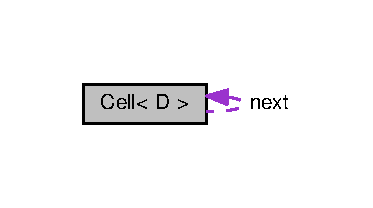
\includegraphics[width=179pt]{classCell__coll__graph}
\end{center}
\end{figure}
\subsection*{Public Member Functions}
\begin{DoxyCompactItemize}
\item 
\hyperlink{classCell_a742a2adf7fa420fa9cbe386a87b5c79b}{Cell} ()
\item 
\hyperlink{classCell_a6724cd6a883d7c16f2f529ecfd0dbf68}{Cell} (D $\ast$\hyperlink{classCell_ab8cc4d3059ef84a652eabc05b6c28f49}{data}, \hyperlink{classCell}{Cell} $\ast$\hyperlink{classCell_a7e0e6c090f8aca70862c2dbc3257e3b9}{next})
\item 
\hyperlink{classCell_a1882f51b9de9f6f52c5fb0530128bc92}{Cell} (const \hyperlink{classCell}{Cell} \&cell)
\item 
virtual \hyperlink{classCell_a8a6091a249d6ff583049c35c85f4d778}{$\sim$\+Cell} ()
\end{DoxyCompactItemize}
\subsection*{Data Fields}
\begin{DoxyCompactItemize}
\item 
\hyperlink{classCell}{Cell} $\ast$ \hyperlink{classCell_a7e0e6c090f8aca70862c2dbc3257e3b9}{next}
\item 
D $\ast$ \hyperlink{classCell_ab8cc4d3059ef84a652eabc05b6c28f49}{data}
\end{DoxyCompactItemize}


\subsection{Constructor \& Destructor Documentation}
\index{Cell@{Cell}!Cell@{Cell}}
\index{Cell@{Cell}!Cell@{Cell}}
\subsubsection[{\texorpdfstring{Cell()}{Cell()}}]{\setlength{\rightskip}{0pt plus 5cm}template$<$typename D $>$ {\bf Cell}$<$ D $>$\+::{\bf Cell} (
\begin{DoxyParamCaption}
{}
\end{DoxyParamCaption}
)\hspace{0.3cm}{\ttfamily [inline]}}\hypertarget{classCell_a742a2adf7fa420fa9cbe386a87b5c79b}{}\label{classCell_a742a2adf7fa420fa9cbe386a87b5c79b}
\index{Cell@{Cell}!Cell@{Cell}}
\index{Cell@{Cell}!Cell@{Cell}}
\subsubsection[{\texorpdfstring{Cell(\+D $\ast$data, Cell $\ast$next)}{Cell(D *data, Cell *next)}}]{\setlength{\rightskip}{0pt plus 5cm}template$<$typename D $>$ {\bf Cell}$<$ D $>$\+::{\bf Cell} (
\begin{DoxyParamCaption}
\item[{D $\ast$}]{data, }
\item[{{\bf Cell}$<$ D $>$ $\ast$}]{next}
\end{DoxyParamCaption}
)\hspace{0.3cm}{\ttfamily [inline]}}\hypertarget{classCell_a6724cd6a883d7c16f2f529ecfd0dbf68}{}\label{classCell_a6724cd6a883d7c16f2f529ecfd0dbf68}
\index{Cell@{Cell}!Cell@{Cell}}
\index{Cell@{Cell}!Cell@{Cell}}
\subsubsection[{\texorpdfstring{Cell(const Cell \&cell)}{Cell(const Cell &cell)}}]{\setlength{\rightskip}{0pt plus 5cm}template$<$typename D $>$ {\bf Cell}$<$ D $>$\+::{\bf Cell} (
\begin{DoxyParamCaption}
\item[{const {\bf Cell}$<$ D $>$ \&}]{cell}
\end{DoxyParamCaption}
)\hspace{0.3cm}{\ttfamily [inline]}}\hypertarget{classCell_a1882f51b9de9f6f52c5fb0530128bc92}{}\label{classCell_a1882f51b9de9f6f52c5fb0530128bc92}
\index{Cell@{Cell}!````~Cell@{$\sim$\+Cell}}
\index{````~Cell@{$\sim$\+Cell}!Cell@{Cell}}
\subsubsection[{\texorpdfstring{$\sim$\+Cell()}{~Cell()}}]{\setlength{\rightskip}{0pt plus 5cm}template$<$typename D $>$ virtual {\bf Cell}$<$ D $>$\+::$\sim${\bf Cell} (
\begin{DoxyParamCaption}
{}
\end{DoxyParamCaption}
)\hspace{0.3cm}{\ttfamily [inline]}, {\ttfamily [virtual]}}\hypertarget{classCell_a8a6091a249d6ff583049c35c85f4d778}{}\label{classCell_a8a6091a249d6ff583049c35c85f4d778}


\subsection{Field Documentation}
\index{Cell@{Cell}!data@{data}}
\index{data@{data}!Cell@{Cell}}
\subsubsection[{\texorpdfstring{data}{data}}]{\setlength{\rightskip}{0pt plus 5cm}template$<$typename D $>$ D$\ast$ {\bf Cell}$<$ D $>$\+::data}\hypertarget{classCell_ab8cc4d3059ef84a652eabc05b6c28f49}{}\label{classCell_ab8cc4d3059ef84a652eabc05b6c28f49}
\index{Cell@{Cell}!next@{next}}
\index{next@{next}!Cell@{Cell}}
\subsubsection[{\texorpdfstring{next}{next}}]{\setlength{\rightskip}{0pt plus 5cm}template$<$typename D $>$ {\bf Cell}$\ast$ {\bf Cell}$<$ D $>$\+::next}\hypertarget{classCell_a7e0e6c090f8aca70862c2dbc3257e3b9}{}\label{classCell_a7e0e6c090f8aca70862c2dbc3257e3b9}


The documentation for this class was generated from the following file\+:\begin{DoxyCompactItemize}
\item 
\hyperlink{Cell_8h}{Cell.\+h}\end{DoxyCompactItemize}

\hypertarget{classList}{}\section{List$<$ D, P $>$ Class Template Reference}
\label{classList}\index{List$<$ D, P $>$@{List$<$ D, P $>$}}


{\ttfamily \#include $<$List.\+h$>$}



Inheritance diagram for List$<$ D, P $>$\+:
\nopagebreak
\begin{figure}[H]
\begin{center}
\leavevmode
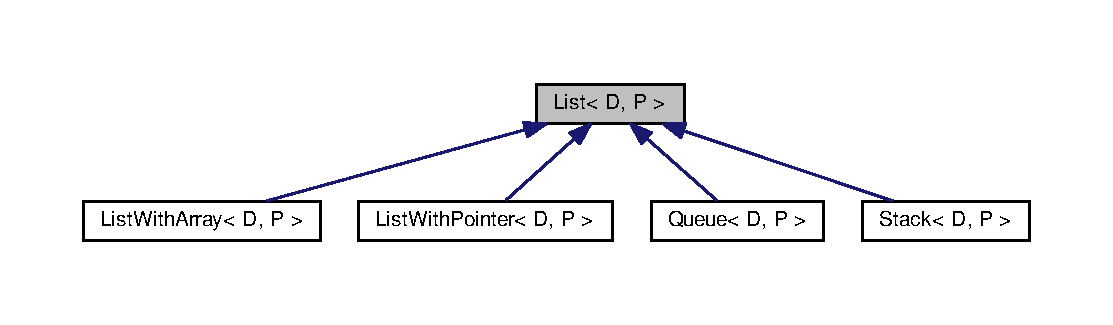
\includegraphics[width=350pt]{classList__inherit__graph}
\end{center}
\end{figure}
\subsection*{Public Member Functions}
\begin{DoxyCompactItemize}
\item 
\hyperlink{classList_a3deb54ab4f51c6c39aa4015f258b5812}{List} ()
\begin{DoxyCompactList}\small\item\em Constructor por defecto. \end{DoxyCompactList}\item 
\hyperlink{classList_af8bcd7dae1bc30af2158075482c3d8d9}{List} (const \hyperlink{classList}{List} \&orig)
\begin{DoxyCompactList}\small\item\em Constructor por copia. \end{DoxyCompactList}\item 
virtual \hyperlink{classList_a624593fb77847bf7ad4cacfba3442471}{$\sim$\+List} ()
\begin{DoxyCompactList}\small\item\em Destructor. \end{DoxyCompactList}\item 
virtual void \hyperlink{classList_a01f588d87d47f8332928eca38f7b11bb}{insert} (D d)=0
\item 
virtual void \hyperlink{classList_a14fc4e853102018df78db3899aa00d71}{remove} (D d)=0
\item 
virtual P \& \hyperlink{classList_ae117dbe387f64f548fd0bddcc4d536dc}{find} (D d)=0
\item 
virtual D \& \hyperlink{classList_afb5a777f30a186adce69028c387bf413}{get} (P \&k)=0
\item 
virtual void \hyperlink{classList_a413440e7e102c944bec31ad5dce30b27}{assign} (P \&k, D d)=0
\item 
virtual void \hyperlink{classList_ae3795939f27cf3e688cd470450e0c27a}{sort} ()=0
\item 
virtual int \hyperlink{classList_af213bbcf13ee436a0f04cde66e337672}{get\+Size} ()=0
\item 
virtual void \hyperlink{classList_a8b34931e187e7e6b86aad86510ce4f3b}{print\+List} ()=0
\item 
virtual P \& \hyperlink{classList_afa9ca2c678bc4f7d15ab0f4ab7c45421}{next} (P \&k)=0
\item 
virtual P \& \hyperlink{classList_a6c44364a04dff392b76e6a286074f3a1}{prev} (P \&k)=0
\item 
virtual void \hyperlink{classList_a24b4f177a70215980e81ef7b2981fa1e}{empty\+List} ()=0
\end{DoxyCompactItemize}
\subsection*{Protected Attributes}
\begin{DoxyCompactItemize}
\item 
int \hyperlink{classList_aa61221b9bda8b2b56a61bd869daacbfd}{n}
\begin{DoxyCompactList}\small\item\em Numero de elementos de la lista. \end{DoxyCompactList}\end{DoxyCompactItemize}


\subsection{Constructor \& Destructor Documentation}
\index{List@{List}!List@{List}}
\index{List@{List}!List@{List}}
\subsubsection[{\texorpdfstring{List()}{List()}}]{\setlength{\rightskip}{0pt plus 5cm}template$<$typename D , typename P $>$ {\bf List}$<$ D, P $>$\+::{\bf List} (
\begin{DoxyParamCaption}
{}
\end{DoxyParamCaption}
)\hspace{0.3cm}{\ttfamily [inline]}}\hypertarget{classList_a3deb54ab4f51c6c39aa4015f258b5812}{}\label{classList_a3deb54ab4f51c6c39aa4015f258b5812}


Constructor por defecto. 

\index{List@{List}!List@{List}}
\index{List@{List}!List@{List}}
\subsubsection[{\texorpdfstring{List(const List \&orig)}{List(const List &orig)}}]{\setlength{\rightskip}{0pt plus 5cm}template$<$typename D , typename P $>$ {\bf List}$<$ D, P $>$\+::{\bf List} (
\begin{DoxyParamCaption}
\item[{const {\bf List}$<$ D, P $>$ \&}]{orig}
\end{DoxyParamCaption}
)\hspace{0.3cm}{\ttfamily [inline]}}\hypertarget{classList_af8bcd7dae1bc30af2158075482c3d8d9}{}\label{classList_af8bcd7dae1bc30af2158075482c3d8d9}


Constructor por copia. 

\index{List@{List}!````~List@{$\sim$\+List}}
\index{````~List@{$\sim$\+List}!List@{List}}
\subsubsection[{\texorpdfstring{$\sim$\+List()}{~List()}}]{\setlength{\rightskip}{0pt plus 5cm}template$<$typename D , typename P $>$ virtual {\bf List}$<$ D, P $>$\+::$\sim${\bf List} (
\begin{DoxyParamCaption}
{}
\end{DoxyParamCaption}
)\hspace{0.3cm}{\ttfamily [inline]}, {\ttfamily [virtual]}}\hypertarget{classList_a624593fb77847bf7ad4cacfba3442471}{}\label{classList_a624593fb77847bf7ad4cacfba3442471}


Destructor. 



\subsection{Member Function Documentation}
\index{List@{List}!assign@{assign}}
\index{assign@{assign}!List@{List}}
\subsubsection[{\texorpdfstring{assign(\+P \&k, D d)=0}{assign(P &k, D d)=0}}]{\setlength{\rightskip}{0pt plus 5cm}template$<$typename D , typename P $>$ virtual void {\bf List}$<$ D, P $>$\+::assign (
\begin{DoxyParamCaption}
\item[{P \&}]{k, }
\item[{D}]{d}
\end{DoxyParamCaption}
)\hspace{0.3cm}{\ttfamily [pure virtual]}}\hypertarget{classList_a413440e7e102c944bec31ad5dce30b27}{}\label{classList_a413440e7e102c944bec31ad5dce30b27}


Implemented in \hyperlink{classListWithPointer_a5703464a7cd48d871e3bb04562a3d351}{List\+With\+Pointer$<$ D, P $>$}, \hyperlink{classStack_a8925b69439c6d583cf0a62f9a0cca026}{Stack$<$ D, P $>$}, \hyperlink{classQueue_af8e5f753e54a7eb2a770c1bbf0c1d8fe}{Queue$<$ D, P $>$}, and \hyperlink{classListWithArray_ad673838a35904292aca7ef78d64fceca}{List\+With\+Array$<$ D, P $>$}.

\index{List@{List}!empty\+List@{empty\+List}}
\index{empty\+List@{empty\+List}!List@{List}}
\subsubsection[{\texorpdfstring{empty\+List()=0}{emptyList()=0}}]{\setlength{\rightskip}{0pt plus 5cm}template$<$typename D , typename P $>$ virtual void {\bf List}$<$ D, P $>$\+::empty\+List (
\begin{DoxyParamCaption}
{}
\end{DoxyParamCaption}
)\hspace{0.3cm}{\ttfamily [pure virtual]}}\hypertarget{classList_a24b4f177a70215980e81ef7b2981fa1e}{}\label{classList_a24b4f177a70215980e81ef7b2981fa1e}


Implemented in \hyperlink{classListWithArray_a2179e228f285cc29b46bd5d13ba0b4ed}{List\+With\+Array$<$ D, P $>$}, \hyperlink{classListWithPointer_aec4f5374971962c79d397bbcd0080199}{List\+With\+Pointer$<$ D, P $>$}, \hyperlink{classStack_a8d4119c8d4be2822f20a525743aa296e}{Stack$<$ D, P $>$}, and \hyperlink{classQueue_a37e23ca9e4ac29be510833bf6b7f6638}{Queue$<$ D, P $>$}.

\index{List@{List}!find@{find}}
\index{find@{find}!List@{List}}
\subsubsection[{\texorpdfstring{find(\+D d)=0}{find(D d)=0}}]{\setlength{\rightskip}{0pt plus 5cm}template$<$typename D , typename P $>$ virtual P\& {\bf List}$<$ D, P $>$\+::find (
\begin{DoxyParamCaption}
\item[{D}]{d}
\end{DoxyParamCaption}
)\hspace{0.3cm}{\ttfamily [pure virtual]}}\hypertarget{classList_ae117dbe387f64f548fd0bddcc4d536dc}{}\label{classList_ae117dbe387f64f548fd0bddcc4d536dc}


Implemented in \hyperlink{classListWithPointer_a28695477b0cfdc456271e31f5e0d6429}{List\+With\+Pointer$<$ D, P $>$}, \hyperlink{classListWithArray_a83d6be27dd1ace1e409df0ba000c9f39}{List\+With\+Array$<$ D, P $>$}, \hyperlink{classQueue_aefef2f172eaa0606944cdb4cf2fd5c53}{Queue$<$ D, P $>$}, and \hyperlink{classStack_a2d24bac6bd65a0c90dd0dbe5c1297c1b}{Stack$<$ D, P $>$}.

\index{List@{List}!get@{get}}
\index{get@{get}!List@{List}}
\subsubsection[{\texorpdfstring{get(\+P \&k)=0}{get(P &k)=0}}]{\setlength{\rightskip}{0pt plus 5cm}template$<$typename D , typename P $>$ virtual D\& {\bf List}$<$ D, P $>$\+::get (
\begin{DoxyParamCaption}
\item[{P \&}]{k}
\end{DoxyParamCaption}
)\hspace{0.3cm}{\ttfamily [pure virtual]}}\hypertarget{classList_afb5a777f30a186adce69028c387bf413}{}\label{classList_afb5a777f30a186adce69028c387bf413}


Implemented in \hyperlink{classListWithPointer_af2892238e8faed0b98d2473419a91f62}{List\+With\+Pointer$<$ D, P $>$}, \hyperlink{classListWithArray_a716a279651d30b3fca9df3506ed77535}{List\+With\+Array$<$ D, P $>$}, \hyperlink{classQueue_a1f2067f6e952bb0cec06087210b5ae2f}{Queue$<$ D, P $>$}, and \hyperlink{classStack_a488e4c5a68c70b5221df734fd953983f}{Stack$<$ D, P $>$}.

\index{List@{List}!get\+Size@{get\+Size}}
\index{get\+Size@{get\+Size}!List@{List}}
\subsubsection[{\texorpdfstring{get\+Size()=0}{getSize()=0}}]{\setlength{\rightskip}{0pt plus 5cm}template$<$typename D , typename P $>$ virtual int {\bf List}$<$ D, P $>$\+::get\+Size (
\begin{DoxyParamCaption}
{}
\end{DoxyParamCaption}
)\hspace{0.3cm}{\ttfamily [pure virtual]}}\hypertarget{classList_af213bbcf13ee436a0f04cde66e337672}{}\label{classList_af213bbcf13ee436a0f04cde66e337672}


Implemented in \hyperlink{classListWithArray_ae7a071bcdde9ddbf4c40a716f5a09434}{List\+With\+Array$<$ D, P $>$}, \hyperlink{classListWithPointer_ac70c49b5703887fd867e90cdac3c706f}{List\+With\+Pointer$<$ D, P $>$}, \hyperlink{classQueue_ab2c7217e6737bf579493b321184a2db3}{Queue$<$ D, P $>$}, and \hyperlink{classStack_a74fc7e5921dfb247f9ad7052c3c4297a}{Stack$<$ D, P $>$}.

\index{List@{List}!insert@{insert}}
\index{insert@{insert}!List@{List}}
\subsubsection[{\texorpdfstring{insert(\+D d)=0}{insert(D d)=0}}]{\setlength{\rightskip}{0pt plus 5cm}template$<$typename D , typename P $>$ virtual void {\bf List}$<$ D, P $>$\+::insert (
\begin{DoxyParamCaption}
\item[{D}]{d}
\end{DoxyParamCaption}
)\hspace{0.3cm}{\ttfamily [pure virtual]}}\hypertarget{classList_a01f588d87d47f8332928eca38f7b11bb}{}\label{classList_a01f588d87d47f8332928eca38f7b11bb}


Implemented in \hyperlink{classListWithArray_afa0b6d215c2cc1d3fe6b9b48d6b6917d}{List\+With\+Array$<$ D, P $>$}, \hyperlink{classListWithPointer_a726958a731ead3b407d68a7e5a0bce54}{List\+With\+Pointer$<$ D, P $>$}, \hyperlink{classQueue_a63bd4d9779ddd75b2f78127337fe786a}{Queue$<$ D, P $>$}, and \hyperlink{classStack_a2d8dfebafe6767cd668bcfc64d33bf63}{Stack$<$ D, P $>$}.

\index{List@{List}!next@{next}}
\index{next@{next}!List@{List}}
\subsubsection[{\texorpdfstring{next(\+P \&k)=0}{next(P &k)=0}}]{\setlength{\rightskip}{0pt plus 5cm}template$<$typename D , typename P $>$ virtual P\& {\bf List}$<$ D, P $>$\+::next (
\begin{DoxyParamCaption}
\item[{P \&}]{k}
\end{DoxyParamCaption}
)\hspace{0.3cm}{\ttfamily [pure virtual]}}\hypertarget{classList_afa9ca2c678bc4f7d15ab0f4ab7c45421}{}\label{classList_afa9ca2c678bc4f7d15ab0f4ab7c45421}


Implemented in \hyperlink{classListWithArray_a65ef8c78e19dfa00e58c3e92f1be6fb1}{List\+With\+Array$<$ D, P $>$}, \hyperlink{classListWithPointer_a3aec82866e03a1f37175c4b0976eeb47}{List\+With\+Pointer$<$ D, P $>$}, \hyperlink{classQueue_a989738789320704ae2d597e73919aefa}{Queue$<$ D, P $>$}, and \hyperlink{classStack_aa86ccdcc6e57ade075de6ee51d1e5341}{Stack$<$ D, P $>$}.

\index{List@{List}!prev@{prev}}
\index{prev@{prev}!List@{List}}
\subsubsection[{\texorpdfstring{prev(\+P \&k)=0}{prev(P &k)=0}}]{\setlength{\rightskip}{0pt plus 5cm}template$<$typename D , typename P $>$ virtual P\& {\bf List}$<$ D, P $>$\+::prev (
\begin{DoxyParamCaption}
\item[{P \&}]{k}
\end{DoxyParamCaption}
)\hspace{0.3cm}{\ttfamily [pure virtual]}}\hypertarget{classList_a6c44364a04dff392b76e6a286074f3a1}{}\label{classList_a6c44364a04dff392b76e6a286074f3a1}


Implemented in \hyperlink{classListWithArray_aee46046c55e1e0ee1f37b5e1a7aa0702}{List\+With\+Array$<$ D, P $>$}, \hyperlink{classListWithPointer_a89f1ef1d78fe7f78290eaab585a14cca}{List\+With\+Pointer$<$ D, P $>$}, \hyperlink{classQueue_a238a908300566b4f9bb379216c7527c6}{Queue$<$ D, P $>$}, and \hyperlink{classStack_a1e45de0c08c059313e99772c9e53820a}{Stack$<$ D, P $>$}.

\index{List@{List}!print\+List@{print\+List}}
\index{print\+List@{print\+List}!List@{List}}
\subsubsection[{\texorpdfstring{print\+List()=0}{printList()=0}}]{\setlength{\rightskip}{0pt plus 5cm}template$<$typename D , typename P $>$ virtual void {\bf List}$<$ D, P $>$\+::print\+List (
\begin{DoxyParamCaption}
{}
\end{DoxyParamCaption}
)\hspace{0.3cm}{\ttfamily [pure virtual]}}\hypertarget{classList_a8b34931e187e7e6b86aad86510ce4f3b}{}\label{classList_a8b34931e187e7e6b86aad86510ce4f3b}


Implemented in \hyperlink{classListWithArray_a515ea38cb40ba7b0c9df98825b2dd270}{List\+With\+Array$<$ D, P $>$}, \hyperlink{classListWithPointer_a7079b5f1dbddb87a7e33ffc71ebb7b92}{List\+With\+Pointer$<$ D, P $>$}, \hyperlink{classQueue_aa461f8fb363f960a6e0eb34b18503eaa}{Queue$<$ D, P $>$}, and \hyperlink{classStack_a89b9967c15c83fe7c257a42e49725881}{Stack$<$ D, P $>$}.

\index{List@{List}!remove@{remove}}
\index{remove@{remove}!List@{List}}
\subsubsection[{\texorpdfstring{remove(\+D d)=0}{remove(D d)=0}}]{\setlength{\rightskip}{0pt plus 5cm}template$<$typename D , typename P $>$ virtual void {\bf List}$<$ D, P $>$\+::remove (
\begin{DoxyParamCaption}
\item[{D}]{d}
\end{DoxyParamCaption}
)\hspace{0.3cm}{\ttfamily [pure virtual]}}\hypertarget{classList_a14fc4e853102018df78db3899aa00d71}{}\label{classList_a14fc4e853102018df78db3899aa00d71}


Implemented in \hyperlink{classListWithArray_aaa18e76fc128ca05151178d914901ec3}{List\+With\+Array$<$ D, P $>$}, \hyperlink{classListWithPointer_ab69e83d9e92619be09f9d8dde3e6cad0}{List\+With\+Pointer$<$ D, P $>$}, \hyperlink{classStack_a44889855bb26c4b1e050668959fab5be}{Stack$<$ D, P $>$}, and \hyperlink{classQueue_aa3d1a6edd30c4a9dda42e586db7f9fff}{Queue$<$ D, P $>$}.

\index{List@{List}!sort@{sort}}
\index{sort@{sort}!List@{List}}
\subsubsection[{\texorpdfstring{sort()=0}{sort()=0}}]{\setlength{\rightskip}{0pt plus 5cm}template$<$typename D , typename P $>$ virtual void {\bf List}$<$ D, P $>$\+::sort (
\begin{DoxyParamCaption}
{}
\end{DoxyParamCaption}
)\hspace{0.3cm}{\ttfamily [pure virtual]}}\hypertarget{classList_ae3795939f27cf3e688cd470450e0c27a}{}\label{classList_ae3795939f27cf3e688cd470450e0c27a}


Implemented in \hyperlink{classListWithPointer_aa46631b2da29895d1f767626fb591bc8}{List\+With\+Pointer$<$ D, P $>$}, \hyperlink{classStack_a75261d2340f1f7b5e61b3770c0550982}{Stack$<$ D, P $>$}, \hyperlink{classQueue_a896b0e1bcac0d660079eb838c1823446}{Queue$<$ D, P $>$}, and \hyperlink{classListWithArray_a1a0ec4ab4a8fcb1a20568445ad892c9a}{List\+With\+Array$<$ D, P $>$}.



\subsection{Field Documentation}
\index{List@{List}!n@{n}}
\index{n@{n}!List@{List}}
\subsubsection[{\texorpdfstring{n}{n}}]{\setlength{\rightskip}{0pt plus 5cm}template$<$typename D , typename P $>$ int {\bf List}$<$ D, P $>$\+::n\hspace{0.3cm}{\ttfamily [protected]}}\hypertarget{classList_aa61221b9bda8b2b56a61bd869daacbfd}{}\label{classList_aa61221b9bda8b2b56a61bd869daacbfd}


Numero de elementos de la lista. 



The documentation for this class was generated from the following file\+:\begin{DoxyCompactItemize}
\item 
\hyperlink{List_8h}{List.\+h}\end{DoxyCompactItemize}

\hypertarget{classListWithArray}{}\section{List\+With\+Array$<$ D, P $>$ Class Template Reference}
\label{classListWithArray}\index{List\+With\+Array$<$ D, P $>$@{List\+With\+Array$<$ D, P $>$}}


{\ttfamily \#include $<$List\+With\+Array.\+h$>$}



Inheritance diagram for List\+With\+Array$<$ D, P $>$\+:
\nopagebreak
\begin{figure}[H]
\begin{center}
\leavevmode
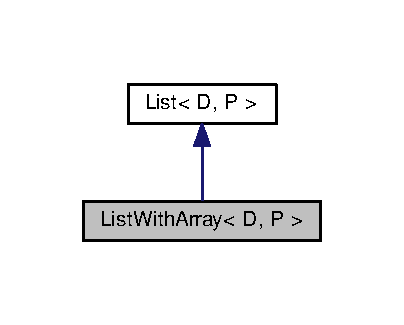
\includegraphics[width=194pt]{classListWithArray__inherit__graph}
\end{center}
\end{figure}


Collaboration diagram for List\+With\+Array$<$ D, P $>$\+:
\nopagebreak
\begin{figure}[H]
\begin{center}
\leavevmode
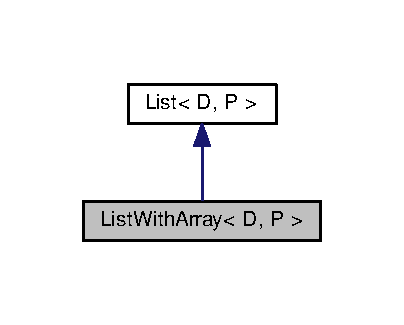
\includegraphics[width=194pt]{classListWithArray__coll__graph}
\end{center}
\end{figure}
\subsection*{Public Member Functions}
\begin{DoxyCompactItemize}
\item 
\hyperlink{classListWithArray_a06f0e8035e9cc43aff4d32c46a00fcf0}{List\+With\+Array} ()
\begin{DoxyCompactList}\small\item\em Constructor por defecto. Se crea con los atributos nulos y n en 0. \end{DoxyCompactList}\item 
\hyperlink{classListWithArray_a3a6d11f203fb0f7e458672e85db26b03}{List\+With\+Array} (int t)
\begin{DoxyCompactList}\small\item\em Constructor para un numero maximo de elementos dados. \end{DoxyCompactList}\item 
\hyperlink{classListWithArray_a760ab3b39abb104e76a1fdbd2d303cc2}{List\+With\+Array} (const \hyperlink{classListWithArray}{List\+With\+Array} \&orig)
\begin{DoxyCompactList}\small\item\em Constructor por copia. \end{DoxyCompactList}\item 
\hyperlink{classListWithArray_a1886482555430b0f3eb5ebe02cbb0c87}{$\sim$\+List\+With\+Array} ()
\begin{DoxyCompactList}\small\item\em Destructor. \end{DoxyCompactList}\item 
void \hyperlink{classListWithArray_afa0b6d215c2cc1d3fe6b9b48d6b6917d}{insert} (D d)
\begin{DoxyCompactList}\small\item\em Metodo para insertar un dato a la lista. El dato insertado se hace al final de la lista. \end{DoxyCompactList}\item 
void \hyperlink{classListWithArray_aaa18e76fc128ca05151178d914901ec3}{remove} (D d)
\begin{DoxyCompactList}\small\item\em Metodo para remueve un dato de la lista. \end{DoxyCompactList}\item 
P \& \hyperlink{classListWithArray_a83d6be27dd1ace1e409df0ba000c9f39}{find} (D d)
\begin{DoxyCompactList}\small\item\em Metodo para encontrar un dato en la lista. \end{DoxyCompactList}\item 
D \& \hyperlink{classListWithArray_a716a279651d30b3fca9df3506ed77535}{get} (P \&k)
\begin{DoxyCompactList}\small\item\em Metodo encontrar el dato de la posicion que se pasa como parametro. \end{DoxyCompactList}\item 
void \hyperlink{classListWithArray_ad673838a35904292aca7ef78d64fceca}{assign} (P \&k, D d)
\begin{DoxyCompactList}\small\item\em Metodo para assignarle el dato d a la posicion k. \end{DoxyCompactList}\item 
void \hyperlink{classListWithArray_a1a0ec4ab4a8fcb1a20568445ad892c9a}{sort} ()
\begin{DoxyCompactList}\small\item\em Metodo para ordenar la lista. Se usa el algoritmo bubble sort. \end{DoxyCompactList}\item 
int \hyperlink{classListWithArray_ae7a071bcdde9ddbf4c40a716f5a09434}{get\+Size} ()
\begin{DoxyCompactList}\small\item\em Metodo para encontrar el tamanno de la lista. \end{DoxyCompactList}\item 
void \hyperlink{classListWithArray_a515ea38cb40ba7b0c9df98825b2dd270}{print\+List} ()
\begin{DoxyCompactList}\small\item\em Metodo para imprimir la lista. \end{DoxyCompactList}\item 
P \& \hyperlink{classListWithArray_a65ef8c78e19dfa00e58c3e92f1be6fb1}{next} (P \&k)
\begin{DoxyCompactList}\small\item\em Metodo para encontrar el dato siguiente a una posicion dada. \end{DoxyCompactList}\item 
P \& \hyperlink{classListWithArray_aee46046c55e1e0ee1f37b5e1a7aa0702}{prev} (P \&k)
\begin{DoxyCompactList}\small\item\em Metodo para encontrar el dato anterior a una posicion dada. \end{DoxyCompactList}\item 
void \hyperlink{classListWithArray_a2179e228f285cc29b46bd5d13ba0b4ed}{empty\+List} ()
\begin{DoxyCompactList}\small\item\em Metodo para vaciar la lista. \end{DoxyCompactList}\end{DoxyCompactItemize}
\subsection*{Additional Inherited Members}


\subsection{Constructor \& Destructor Documentation}
\index{List\+With\+Array@{List\+With\+Array}!List\+With\+Array@{List\+With\+Array}}
\index{List\+With\+Array@{List\+With\+Array}!List\+With\+Array@{List\+With\+Array}}
\subsubsection[{\texorpdfstring{List\+With\+Array()}{ListWithArray()}}]{\setlength{\rightskip}{0pt plus 5cm}template$<$typename D , typename P $>$ {\bf List\+With\+Array}$<$ D, P $>$\+::{\bf List\+With\+Array} (
\begin{DoxyParamCaption}
{}
\end{DoxyParamCaption}
)\hspace{0.3cm}{\ttfamily [inline]}}\hypertarget{classListWithArray_a06f0e8035e9cc43aff4d32c46a00fcf0}{}\label{classListWithArray_a06f0e8035e9cc43aff4d32c46a00fcf0}


Constructor por defecto. Se crea con los atributos nulos y n en 0. 

\index{List\+With\+Array@{List\+With\+Array}!List\+With\+Array@{List\+With\+Array}}
\index{List\+With\+Array@{List\+With\+Array}!List\+With\+Array@{List\+With\+Array}}
\subsubsection[{\texorpdfstring{List\+With\+Array(int t)}{ListWithArray(int t)}}]{\setlength{\rightskip}{0pt plus 5cm}template$<$typename D , typename P $>$ {\bf List\+With\+Array}$<$ D, P $>$\+::{\bf List\+With\+Array} (
\begin{DoxyParamCaption}
\item[{int}]{t}
\end{DoxyParamCaption}
)\hspace{0.3cm}{\ttfamily [inline]}}\hypertarget{classListWithArray_a3a6d11f203fb0f7e458672e85db26b03}{}\label{classListWithArray_a3a6d11f203fb0f7e458672e85db26b03}


Constructor para un numero maximo de elementos dados. 

\index{List\+With\+Array@{List\+With\+Array}!List\+With\+Array@{List\+With\+Array}}
\index{List\+With\+Array@{List\+With\+Array}!List\+With\+Array@{List\+With\+Array}}
\subsubsection[{\texorpdfstring{List\+With\+Array(const List\+With\+Array \&orig)}{ListWithArray(const ListWithArray &orig)}}]{\setlength{\rightskip}{0pt plus 5cm}template$<$typename D , typename P $>$ {\bf List\+With\+Array}$<$ D, P $>$\+::{\bf List\+With\+Array} (
\begin{DoxyParamCaption}
\item[{const {\bf List\+With\+Array}$<$ D, P $>$ \&}]{orig}
\end{DoxyParamCaption}
)\hspace{0.3cm}{\ttfamily [inline]}}\hypertarget{classListWithArray_a760ab3b39abb104e76a1fdbd2d303cc2}{}\label{classListWithArray_a760ab3b39abb104e76a1fdbd2d303cc2}


Constructor por copia. 

\index{List\+With\+Array@{List\+With\+Array}!````~List\+With\+Array@{$\sim$\+List\+With\+Array}}
\index{````~List\+With\+Array@{$\sim$\+List\+With\+Array}!List\+With\+Array@{List\+With\+Array}}
\subsubsection[{\texorpdfstring{$\sim$\+List\+With\+Array()}{~ListWithArray()}}]{\setlength{\rightskip}{0pt plus 5cm}template$<$typename D , typename P $>$ {\bf List\+With\+Array}$<$ D, P $>$\+::$\sim${\bf List\+With\+Array} (
\begin{DoxyParamCaption}
{}
\end{DoxyParamCaption}
)\hspace{0.3cm}{\ttfamily [inline]}}\hypertarget{classListWithArray_a1886482555430b0f3eb5ebe02cbb0c87}{}\label{classListWithArray_a1886482555430b0f3eb5ebe02cbb0c87}


Destructor. 



\subsection{Member Function Documentation}
\index{List\+With\+Array@{List\+With\+Array}!assign@{assign}}
\index{assign@{assign}!List\+With\+Array@{List\+With\+Array}}
\subsubsection[{\texorpdfstring{assign(\+P \&k, D d)}{assign(P &k, D d)}}]{\setlength{\rightskip}{0pt plus 5cm}template$<$typename D , typename P $>$ void {\bf List\+With\+Array}$<$ D, P $>$\+::assign (
\begin{DoxyParamCaption}
\item[{P \&}]{k, }
\item[{D}]{d}
\end{DoxyParamCaption}
)\hspace{0.3cm}{\ttfamily [inline]}, {\ttfamily [virtual]}}\hypertarget{classListWithArray_ad673838a35904292aca7ef78d64fceca}{}\label{classListWithArray_ad673838a35904292aca7ef78d64fceca}


Metodo para assignarle el dato d a la posicion k. 


\begin{DoxyParams}{Parameters}
{\em d} & El dato que se quiere asignar. \\
\hline
{\em k} & Posicion a la que se le quiere asignar este dato. \\
\hline
\end{DoxyParams}


Implements \hyperlink{classList_a413440e7e102c944bec31ad5dce30b27}{List$<$ D, P $>$}.

\index{List\+With\+Array@{List\+With\+Array}!empty\+List@{empty\+List}}
\index{empty\+List@{empty\+List}!List\+With\+Array@{List\+With\+Array}}
\subsubsection[{\texorpdfstring{empty\+List()}{emptyList()}}]{\setlength{\rightskip}{0pt plus 5cm}template$<$typename D , typename P $>$ void {\bf List\+With\+Array}$<$ D, P $>$\+::empty\+List (
\begin{DoxyParamCaption}
{}
\end{DoxyParamCaption}
)\hspace{0.3cm}{\ttfamily [inline]}, {\ttfamily [virtual]}}\hypertarget{classListWithArray_a2179e228f285cc29b46bd5d13ba0b4ed}{}\label{classListWithArray_a2179e228f285cc29b46bd5d13ba0b4ed}


Metodo para vaciar la lista. 



Implements \hyperlink{classList_a24b4f177a70215980e81ef7b2981fa1e}{List$<$ D, P $>$}.

\index{List\+With\+Array@{List\+With\+Array}!find@{find}}
\index{find@{find}!List\+With\+Array@{List\+With\+Array}}
\subsubsection[{\texorpdfstring{find(\+D d)}{find(D d)}}]{\setlength{\rightskip}{0pt plus 5cm}template$<$typename D , typename P $>$ P\& {\bf List\+With\+Array}$<$ D, P $>$\+::find (
\begin{DoxyParamCaption}
\item[{D}]{d}
\end{DoxyParamCaption}
)\hspace{0.3cm}{\ttfamily [inline]}, {\ttfamily [virtual]}}\hypertarget{classListWithArray_a83d6be27dd1ace1e409df0ba000c9f39}{}\label{classListWithArray_a83d6be27dd1ace1e409df0ba000c9f39}


Metodo para encontrar un dato en la lista. 


\begin{DoxyParams}{Parameters}
{\em d} & Dato que queremos encontrar. \\
\hline
\end{DoxyParams}
\begin{DoxyReturn}{Returns}
Referencia de la posicion que contiene dicho dato. 
\end{DoxyReturn}


Implements \hyperlink{classList_ae117dbe387f64f548fd0bddcc4d536dc}{List$<$ D, P $>$}.

\index{List\+With\+Array@{List\+With\+Array}!get@{get}}
\index{get@{get}!List\+With\+Array@{List\+With\+Array}}
\subsubsection[{\texorpdfstring{get(\+P \&k)}{get(P &k)}}]{\setlength{\rightskip}{0pt plus 5cm}template$<$typename D , typename P $>$ D\& {\bf List\+With\+Array}$<$ D, P $>$\+::get (
\begin{DoxyParamCaption}
\item[{P \&}]{k}
\end{DoxyParamCaption}
)\hspace{0.3cm}{\ttfamily [inline]}, {\ttfamily [virtual]}}\hypertarget{classListWithArray_a716a279651d30b3fca9df3506ed77535}{}\label{classListWithArray_a716a279651d30b3fca9df3506ed77535}


Metodo encontrar el dato de la posicion que se pasa como parametro. 


\begin{DoxyParams}{Parameters}
{\em k} & La celda de la cual ocupamos encontrar el dato. \\
\hline
\end{DoxyParams}
\begin{DoxyReturn}{Returns}
Referencia del dato que contiene la posicion. 
\end{DoxyReturn}


Implements \hyperlink{classList_afb5a777f30a186adce69028c387bf413}{List$<$ D, P $>$}.

\index{List\+With\+Array@{List\+With\+Array}!get\+Size@{get\+Size}}
\index{get\+Size@{get\+Size}!List\+With\+Array@{List\+With\+Array}}
\subsubsection[{\texorpdfstring{get\+Size()}{getSize()}}]{\setlength{\rightskip}{0pt plus 5cm}template$<$typename D , typename P $>$ int {\bf List\+With\+Array}$<$ D, P $>$\+::get\+Size (
\begin{DoxyParamCaption}
{}
\end{DoxyParamCaption}
)\hspace{0.3cm}{\ttfamily [inline]}, {\ttfamily [virtual]}}\hypertarget{classListWithArray_ae7a071bcdde9ddbf4c40a716f5a09434}{}\label{classListWithArray_ae7a071bcdde9ddbf4c40a716f5a09434}


Metodo para encontrar el tamanno de la lista. 

\begin{DoxyReturn}{Returns}
Un entero con el numero de elementos que tiene la lista. 
\end{DoxyReturn}


Implements \hyperlink{classList_af213bbcf13ee436a0f04cde66e337672}{List$<$ D, P $>$}.

\index{List\+With\+Array@{List\+With\+Array}!insert@{insert}}
\index{insert@{insert}!List\+With\+Array@{List\+With\+Array}}
\subsubsection[{\texorpdfstring{insert(\+D d)}{insert(D d)}}]{\setlength{\rightskip}{0pt plus 5cm}template$<$typename D , typename P $>$ void {\bf List\+With\+Array}$<$ D, P $>$\+::insert (
\begin{DoxyParamCaption}
\item[{D}]{d}
\end{DoxyParamCaption}
)\hspace{0.3cm}{\ttfamily [inline]}, {\ttfamily [virtual]}}\hypertarget{classListWithArray_afa0b6d215c2cc1d3fe6b9b48d6b6917d}{}\label{classListWithArray_afa0b6d215c2cc1d3fe6b9b48d6b6917d}


Metodo para insertar un dato a la lista. El dato insertado se hace al final de la lista. 


\begin{DoxyParams}{Parameters}
{\em d} & El dato que se quiere insertar. \\
\hline
\end{DoxyParams}


Implements \hyperlink{classList_a01f588d87d47f8332928eca38f7b11bb}{List$<$ D, P $>$}.

\index{List\+With\+Array@{List\+With\+Array}!next@{next}}
\index{next@{next}!List\+With\+Array@{List\+With\+Array}}
\subsubsection[{\texorpdfstring{next(\+P \&k)}{next(P &k)}}]{\setlength{\rightskip}{0pt plus 5cm}template$<$typename D , typename P $>$ P\& {\bf List\+With\+Array}$<$ D, P $>$\+::next (
\begin{DoxyParamCaption}
\item[{P \&}]{k}
\end{DoxyParamCaption}
)\hspace{0.3cm}{\ttfamily [inline]}, {\ttfamily [virtual]}}\hypertarget{classListWithArray_a65ef8c78e19dfa00e58c3e92f1be6fb1}{}\label{classListWithArray_a65ef8c78e19dfa00e58c3e92f1be6fb1}


Metodo para encontrar el dato siguiente a una posicion dada. 


\begin{DoxyParams}{Parameters}
{\em k} & La posicion de la cual se quiere el dato siguiente. \\
\hline
\end{DoxyParams}
\begin{DoxyReturn}{Returns}
Referencia de la posicion siguiente. 
\end{DoxyReturn}


Implements \hyperlink{classList_afa9ca2c678bc4f7d15ab0f4ab7c45421}{List$<$ D, P $>$}.

\index{List\+With\+Array@{List\+With\+Array}!prev@{prev}}
\index{prev@{prev}!List\+With\+Array@{List\+With\+Array}}
\subsubsection[{\texorpdfstring{prev(\+P \&k)}{prev(P &k)}}]{\setlength{\rightskip}{0pt plus 5cm}template$<$typename D , typename P $>$ P\& {\bf List\+With\+Array}$<$ D, P $>$\+::prev (
\begin{DoxyParamCaption}
\item[{P \&}]{k}
\end{DoxyParamCaption}
)\hspace{0.3cm}{\ttfamily [inline]}, {\ttfamily [virtual]}}\hypertarget{classListWithArray_aee46046c55e1e0ee1f37b5e1a7aa0702}{}\label{classListWithArray_aee46046c55e1e0ee1f37b5e1a7aa0702}


Metodo para encontrar el dato anterior a una posicion dada. 


\begin{DoxyParams}{Parameters}
{\em k} & La posicion de la cual se quiere el dato anterior. \\
\hline
\end{DoxyParams}
\begin{DoxyReturn}{Returns}
Referencia de la posicion anterior. 
\end{DoxyReturn}


Implements \hyperlink{classList_a6c44364a04dff392b76e6a286074f3a1}{List$<$ D, P $>$}.

\index{List\+With\+Array@{List\+With\+Array}!print\+List@{print\+List}}
\index{print\+List@{print\+List}!List\+With\+Array@{List\+With\+Array}}
\subsubsection[{\texorpdfstring{print\+List()}{printList()}}]{\setlength{\rightskip}{0pt plus 5cm}template$<$typename D , typename P $>$ void {\bf List\+With\+Array}$<$ D, P $>$\+::print\+List (
\begin{DoxyParamCaption}
{}
\end{DoxyParamCaption}
)\hspace{0.3cm}{\ttfamily [inline]}, {\ttfamily [virtual]}}\hypertarget{classListWithArray_a515ea38cb40ba7b0c9df98825b2dd270}{}\label{classListWithArray_a515ea38cb40ba7b0c9df98825b2dd270}


Metodo para imprimir la lista. 



Implements \hyperlink{classList_a8b34931e187e7e6b86aad86510ce4f3b}{List$<$ D, P $>$}.

\index{List\+With\+Array@{List\+With\+Array}!remove@{remove}}
\index{remove@{remove}!List\+With\+Array@{List\+With\+Array}}
\subsubsection[{\texorpdfstring{remove(\+D d)}{remove(D d)}}]{\setlength{\rightskip}{0pt plus 5cm}template$<$typename D , typename P $>$ void {\bf List\+With\+Array}$<$ D, P $>$\+::remove (
\begin{DoxyParamCaption}
\item[{D}]{d}
\end{DoxyParamCaption}
)\hspace{0.3cm}{\ttfamily [inline]}, {\ttfamily [virtual]}}\hypertarget{classListWithArray_aaa18e76fc128ca05151178d914901ec3}{}\label{classListWithArray_aaa18e76fc128ca05151178d914901ec3}


Metodo para remueve un dato de la lista. 


\begin{DoxyParams}{Parameters}
{\em d} & El dato que debe contener la cela a eliminar. \\
\hline
\end{DoxyParams}


Implements \hyperlink{classList_a14fc4e853102018df78db3899aa00d71}{List$<$ D, P $>$}.

\index{List\+With\+Array@{List\+With\+Array}!sort@{sort}}
\index{sort@{sort}!List\+With\+Array@{List\+With\+Array}}
\subsubsection[{\texorpdfstring{sort()}{sort()}}]{\setlength{\rightskip}{0pt plus 5cm}template$<$typename D , typename P $>$ void {\bf List\+With\+Array}$<$ D, P $>$\+::sort (
\begin{DoxyParamCaption}
{}
\end{DoxyParamCaption}
)\hspace{0.3cm}{\ttfamily [inline]}, {\ttfamily [virtual]}}\hypertarget{classListWithArray_a1a0ec4ab4a8fcb1a20568445ad892c9a}{}\label{classListWithArray_a1a0ec4ab4a8fcb1a20568445ad892c9a}


Metodo para ordenar la lista. Se usa el algoritmo bubble sort. 



Implements \hyperlink{classList_ae3795939f27cf3e688cd470450e0c27a}{List$<$ D, P $>$}.



The documentation for this class was generated from the following file\+:\begin{DoxyCompactItemize}
\item 
\hyperlink{ListWithArray_8h}{List\+With\+Array.\+h}\end{DoxyCompactItemize}

\hypertarget{classListWithPointer}{}\section{List\+With\+Pointer$<$ D, P $>$ Class Template Reference}
\label{classListWithPointer}\index{List\+With\+Pointer$<$ D, P $>$@{List\+With\+Pointer$<$ D, P $>$}}


{\ttfamily \#include $<$List\+With\+Pointer.\+h$>$}



Inheritance diagram for List\+With\+Pointer$<$ D, P $>$\+:
\nopagebreak
\begin{figure}[H]
\begin{center}
\leavevmode
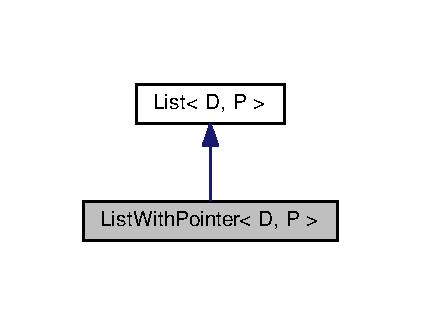
\includegraphics[width=202pt]{classListWithPointer__inherit__graph}
\end{center}
\end{figure}


Collaboration diagram for List\+With\+Pointer$<$ D, P $>$\+:
\nopagebreak
\begin{figure}[H]
\begin{center}
\leavevmode
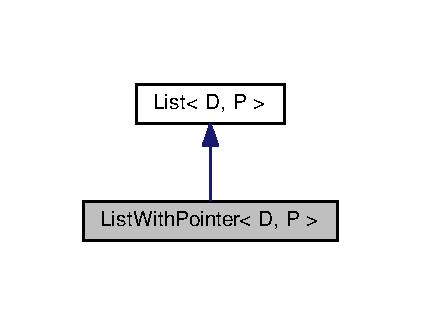
\includegraphics[width=202pt]{classListWithPointer__coll__graph}
\end{center}
\end{figure}
\subsection*{Public Member Functions}
\begin{DoxyCompactItemize}
\item 
\hyperlink{classListWithPointer_a53b1284b13bf834bc5fc1eb27368a283}{List\+With\+Pointer} ()
\item 
virtual \hyperlink{classListWithPointer_ac0567286c62e3521fa5130f95010e779}{$\sim$\+List\+With\+Pointer} ()
\item 
void \hyperlink{classListWithPointer_a726958a731ead3b407d68a7e5a0bce54}{insert} (D data)
\item 
void \hyperlink{classListWithPointer_ab69e83d9e92619be09f9d8dde3e6cad0}{remove} (D data)
\item 
P \hyperlink{classListWithPointer_a2bb95a28a394bffd52a7f962cdde14dd}{find} (D data)
\item 
D \& \hyperlink{classListWithPointer_af2892238e8faed0b98d2473419a91f62}{get} (P \&cell)
\item 
int \hyperlink{classListWithPointer_ac70c49b5703887fd867e90cdac3c706f}{get\+Size} ()
\item 
void \hyperlink{classListWithPointer_a7079b5f1dbddb87a7e33ffc71ebb7b92}{print\+List} ()
\item 
P \& \hyperlink{classListWithPointer_a3aec82866e03a1f37175c4b0976eeb47}{next} (P \&cell)
\item 
P \hyperlink{classListWithPointer_ab3b37e6a31e0837884b91df6da682cc8}{prev} (P cell)
\item 
void \hyperlink{classListWithPointer_aec4f5374971962c79d397bbcd0080199}{empty\+List} ()
\item 
void \hyperlink{classListWithPointer_a0727a8a01df92681f13a74acd8dc2247}{erase} (P $\ast$k)
\item 
void \hyperlink{classListWithPointer_a5703464a7cd48d871e3bb04562a3d351}{assign} (P \&k, D d)
\item 
void \hyperlink{classListWithPointer_ab9cc0d6da9b9e1d40bb57c664a6477cd}{test\+Assign} ()
\item 
void \hyperlink{classListWithPointer_aa46631b2da29895d1f767626fb591bc8}{sort} ()
\item 
D \hyperlink{classListWithPointer_a6b404e952a0b924fc60f7d576a368421}{get\+Last} ()
\item 
D \hyperlink{classListWithPointer_a3fa92037b76b6fd3fb8c9702244eb7fb}{get\+Data\+Pos} (int pos)
\end{DoxyCompactItemize}
\subsection*{Data Fields}
\begin{DoxyCompactItemize}
\item 
P $\ast$ \hyperlink{classListWithPointer_a4d39ded7ea1ef992576f70a933414e12}{first}
\item 
P $\ast$ \hyperlink{classListWithPointer_a639d3b9eba9d217b59b19aaa59b291a7}{last}
\end{DoxyCompactItemize}


\subsection{Constructor \& Destructor Documentation}
\index{List\+With\+Pointer@{List\+With\+Pointer}!List\+With\+Pointer@{List\+With\+Pointer}}
\index{List\+With\+Pointer@{List\+With\+Pointer}!List\+With\+Pointer@{List\+With\+Pointer}}
\subsubsection[{\texorpdfstring{List\+With\+Pointer()}{ListWithPointer()}}]{\setlength{\rightskip}{0pt plus 5cm}template$<$typename D , typename P $>$ {\bf List\+With\+Pointer}$<$ D, P $>$\+::{\bf List\+With\+Pointer} (
\begin{DoxyParamCaption}
{}
\end{DoxyParamCaption}
)\hspace{0.3cm}{\ttfamily [inline]}}\hypertarget{classListWithPointer_a53b1284b13bf834bc5fc1eb27368a283}{}\label{classListWithPointer_a53b1284b13bf834bc5fc1eb27368a283}
\index{List\+With\+Pointer@{List\+With\+Pointer}!````~List\+With\+Pointer@{$\sim$\+List\+With\+Pointer}}
\index{````~List\+With\+Pointer@{$\sim$\+List\+With\+Pointer}!List\+With\+Pointer@{List\+With\+Pointer}}
\subsubsection[{\texorpdfstring{$\sim$\+List\+With\+Pointer()}{~ListWithPointer()}}]{\setlength{\rightskip}{0pt plus 5cm}template$<$typename D , typename P $>$ virtual {\bf List\+With\+Pointer}$<$ D, P $>$\+::$\sim${\bf List\+With\+Pointer} (
\begin{DoxyParamCaption}
{}
\end{DoxyParamCaption}
)\hspace{0.3cm}{\ttfamily [inline]}, {\ttfamily [virtual]}}\hypertarget{classListWithPointer_ac0567286c62e3521fa5130f95010e779}{}\label{classListWithPointer_ac0567286c62e3521fa5130f95010e779}


\subsection{Member Function Documentation}
\index{List\+With\+Pointer@{List\+With\+Pointer}!assign@{assign}}
\index{assign@{assign}!List\+With\+Pointer@{List\+With\+Pointer}}
\subsubsection[{\texorpdfstring{assign(\+P \&k, D d)}{assign(P &k, D d)}}]{\setlength{\rightskip}{0pt plus 5cm}template$<$typename D , typename P $>$ void {\bf List\+With\+Pointer}$<$ D, P $>$\+::assign (
\begin{DoxyParamCaption}
\item[{P \&}]{k, }
\item[{D}]{d}
\end{DoxyParamCaption}
)\hspace{0.3cm}{\ttfamily [inline]}, {\ttfamily [virtual]}}\hypertarget{classListWithPointer_a5703464a7cd48d871e3bb04562a3d351}{}\label{classListWithPointer_a5703464a7cd48d871e3bb04562a3d351}


Implements \hyperlink{classList_a413440e7e102c944bec31ad5dce30b27}{List$<$ D, P $>$}.

\index{List\+With\+Pointer@{List\+With\+Pointer}!empty\+List@{empty\+List}}
\index{empty\+List@{empty\+List}!List\+With\+Pointer@{List\+With\+Pointer}}
\subsubsection[{\texorpdfstring{empty\+List()}{emptyList()}}]{\setlength{\rightskip}{0pt plus 5cm}template$<$typename D , typename P $>$ void {\bf List\+With\+Pointer}$<$ D, P $>$\+::empty\+List (
\begin{DoxyParamCaption}
{}
\end{DoxyParamCaption}
)\hspace{0.3cm}{\ttfamily [inline]}, {\ttfamily [virtual]}}\hypertarget{classListWithPointer_aec4f5374971962c79d397bbcd0080199}{}\label{classListWithPointer_aec4f5374971962c79d397bbcd0080199}


Implements \hyperlink{classList_a24b4f177a70215980e81ef7b2981fa1e}{List$<$ D, P $>$}.

\index{List\+With\+Pointer@{List\+With\+Pointer}!erase@{erase}}
\index{erase@{erase}!List\+With\+Pointer@{List\+With\+Pointer}}
\subsubsection[{\texorpdfstring{erase(\+P $\ast$k)}{erase(P *k)}}]{\setlength{\rightskip}{0pt plus 5cm}template$<$typename D , typename P $>$ void {\bf List\+With\+Pointer}$<$ D, P $>$\+::erase (
\begin{DoxyParamCaption}
\item[{P $\ast$}]{k}
\end{DoxyParamCaption}
)\hspace{0.3cm}{\ttfamily [inline]}}\hypertarget{classListWithPointer_a0727a8a01df92681f13a74acd8dc2247}{}\label{classListWithPointer_a0727a8a01df92681f13a74acd8dc2247}
\index{List\+With\+Pointer@{List\+With\+Pointer}!find@{find}}
\index{find@{find}!List\+With\+Pointer@{List\+With\+Pointer}}
\subsubsection[{\texorpdfstring{find(\+D data)}{find(D data)}}]{\setlength{\rightskip}{0pt plus 5cm}template$<$typename D , typename P $>$ P {\bf List\+With\+Pointer}$<$ D, P $>$\+::find (
\begin{DoxyParamCaption}
\item[{D}]{data}
\end{DoxyParamCaption}
)\hspace{0.3cm}{\ttfamily [inline]}, {\ttfamily [virtual]}}\hypertarget{classListWithPointer_a2bb95a28a394bffd52a7f962cdde14dd}{}\label{classListWithPointer_a2bb95a28a394bffd52a7f962cdde14dd}


Implements \hyperlink{classList_a2b40d6fffc7b2fb5138b648f52c839ee}{List$<$ D, P $>$}.

\index{List\+With\+Pointer@{List\+With\+Pointer}!get@{get}}
\index{get@{get}!List\+With\+Pointer@{List\+With\+Pointer}}
\subsubsection[{\texorpdfstring{get(\+P \&cell)}{get(P &cell)}}]{\setlength{\rightskip}{0pt plus 5cm}template$<$typename D , typename P $>$ D\& {\bf List\+With\+Pointer}$<$ D, P $>$\+::get (
\begin{DoxyParamCaption}
\item[{P \&}]{cell}
\end{DoxyParamCaption}
)\hspace{0.3cm}{\ttfamily [inline]}, {\ttfamily [virtual]}}\hypertarget{classListWithPointer_af2892238e8faed0b98d2473419a91f62}{}\label{classListWithPointer_af2892238e8faed0b98d2473419a91f62}


Implements \hyperlink{classList_afb5a777f30a186adce69028c387bf413}{List$<$ D, P $>$}.

\index{List\+With\+Pointer@{List\+With\+Pointer}!get\+Data\+Pos@{get\+Data\+Pos}}
\index{get\+Data\+Pos@{get\+Data\+Pos}!List\+With\+Pointer@{List\+With\+Pointer}}
\subsubsection[{\texorpdfstring{get\+Data\+Pos(int pos)}{getDataPos(int pos)}}]{\setlength{\rightskip}{0pt plus 5cm}template$<$typename D , typename P $>$ D {\bf List\+With\+Pointer}$<$ D, P $>$\+::get\+Data\+Pos (
\begin{DoxyParamCaption}
\item[{int}]{pos}
\end{DoxyParamCaption}
)\hspace{0.3cm}{\ttfamily [inline]}}\hypertarget{classListWithPointer_a3fa92037b76b6fd3fb8c9702244eb7fb}{}\label{classListWithPointer_a3fa92037b76b6fd3fb8c9702244eb7fb}
\index{List\+With\+Pointer@{List\+With\+Pointer}!get\+Last@{get\+Last}}
\index{get\+Last@{get\+Last}!List\+With\+Pointer@{List\+With\+Pointer}}
\subsubsection[{\texorpdfstring{get\+Last()}{getLast()}}]{\setlength{\rightskip}{0pt plus 5cm}template$<$typename D , typename P $>$ D {\bf List\+With\+Pointer}$<$ D, P $>$\+::get\+Last (
\begin{DoxyParamCaption}
{}
\end{DoxyParamCaption}
)\hspace{0.3cm}{\ttfamily [inline]}}\hypertarget{classListWithPointer_a6b404e952a0b924fc60f7d576a368421}{}\label{classListWithPointer_a6b404e952a0b924fc60f7d576a368421}
\index{List\+With\+Pointer@{List\+With\+Pointer}!get\+Size@{get\+Size}}
\index{get\+Size@{get\+Size}!List\+With\+Pointer@{List\+With\+Pointer}}
\subsubsection[{\texorpdfstring{get\+Size()}{getSize()}}]{\setlength{\rightskip}{0pt plus 5cm}template$<$typename D , typename P $>$ int {\bf List\+With\+Pointer}$<$ D, P $>$\+::get\+Size (
\begin{DoxyParamCaption}
{}
\end{DoxyParamCaption}
)\hspace{0.3cm}{\ttfamily [inline]}, {\ttfamily [virtual]}}\hypertarget{classListWithPointer_ac70c49b5703887fd867e90cdac3c706f}{}\label{classListWithPointer_ac70c49b5703887fd867e90cdac3c706f}


Implements \hyperlink{classList_af213bbcf13ee436a0f04cde66e337672}{List$<$ D, P $>$}.

\index{List\+With\+Pointer@{List\+With\+Pointer}!insert@{insert}}
\index{insert@{insert}!List\+With\+Pointer@{List\+With\+Pointer}}
\subsubsection[{\texorpdfstring{insert(\+D data)}{insert(D data)}}]{\setlength{\rightskip}{0pt plus 5cm}template$<$typename D , typename P $>$ void {\bf List\+With\+Pointer}$<$ D, P $>$\+::insert (
\begin{DoxyParamCaption}
\item[{D}]{data}
\end{DoxyParamCaption}
)\hspace{0.3cm}{\ttfamily [inline]}, {\ttfamily [virtual]}}\hypertarget{classListWithPointer_a726958a731ead3b407d68a7e5a0bce54}{}\label{classListWithPointer_a726958a731ead3b407d68a7e5a0bce54}


Implements \hyperlink{classList_a01f588d87d47f8332928eca38f7b11bb}{List$<$ D, P $>$}.

\index{List\+With\+Pointer@{List\+With\+Pointer}!next@{next}}
\index{next@{next}!List\+With\+Pointer@{List\+With\+Pointer}}
\subsubsection[{\texorpdfstring{next(\+P \&cell)}{next(P &cell)}}]{\setlength{\rightskip}{0pt plus 5cm}template$<$typename D , typename P $>$ P\& {\bf List\+With\+Pointer}$<$ D, P $>$\+::next (
\begin{DoxyParamCaption}
\item[{P \&}]{cell}
\end{DoxyParamCaption}
)\hspace{0.3cm}{\ttfamily [inline]}, {\ttfamily [virtual]}}\hypertarget{classListWithPointer_a3aec82866e03a1f37175c4b0976eeb47}{}\label{classListWithPointer_a3aec82866e03a1f37175c4b0976eeb47}


Implements \hyperlink{classList_afa9ca2c678bc4f7d15ab0f4ab7c45421}{List$<$ D, P $>$}.

\index{List\+With\+Pointer@{List\+With\+Pointer}!prev@{prev}}
\index{prev@{prev}!List\+With\+Pointer@{List\+With\+Pointer}}
\subsubsection[{\texorpdfstring{prev(\+P cell)}{prev(P cell)}}]{\setlength{\rightskip}{0pt plus 5cm}template$<$typename D , typename P $>$ P {\bf List\+With\+Pointer}$<$ D, P $>$\+::prev (
\begin{DoxyParamCaption}
\item[{P}]{cell}
\end{DoxyParamCaption}
)\hspace{0.3cm}{\ttfamily [inline]}, {\ttfamily [virtual]}}\hypertarget{classListWithPointer_ab3b37e6a31e0837884b91df6da682cc8}{}\label{classListWithPointer_ab3b37e6a31e0837884b91df6da682cc8}


Implements \hyperlink{classList_acc1831ae92a288345ef20cb29f3846b2}{List$<$ D, P $>$}.

\index{List\+With\+Pointer@{List\+With\+Pointer}!print\+List@{print\+List}}
\index{print\+List@{print\+List}!List\+With\+Pointer@{List\+With\+Pointer}}
\subsubsection[{\texorpdfstring{print\+List()}{printList()}}]{\setlength{\rightskip}{0pt plus 5cm}template$<$typename D , typename P $>$ void {\bf List\+With\+Pointer}$<$ D, P $>$\+::print\+List (
\begin{DoxyParamCaption}
{}
\end{DoxyParamCaption}
)\hspace{0.3cm}{\ttfamily [inline]}, {\ttfamily [virtual]}}\hypertarget{classListWithPointer_a7079b5f1dbddb87a7e33ffc71ebb7b92}{}\label{classListWithPointer_a7079b5f1dbddb87a7e33ffc71ebb7b92}


Implements \hyperlink{classList_a8b34931e187e7e6b86aad86510ce4f3b}{List$<$ D, P $>$}.

\index{List\+With\+Pointer@{List\+With\+Pointer}!remove@{remove}}
\index{remove@{remove}!List\+With\+Pointer@{List\+With\+Pointer}}
\subsubsection[{\texorpdfstring{remove(\+D data)}{remove(D data)}}]{\setlength{\rightskip}{0pt plus 5cm}template$<$typename D , typename P $>$ void {\bf List\+With\+Pointer}$<$ D, P $>$\+::remove (
\begin{DoxyParamCaption}
\item[{D}]{data}
\end{DoxyParamCaption}
)\hspace{0.3cm}{\ttfamily [inline]}, {\ttfamily [virtual]}}\hypertarget{classListWithPointer_ab69e83d9e92619be09f9d8dde3e6cad0}{}\label{classListWithPointer_ab69e83d9e92619be09f9d8dde3e6cad0}


Implements \hyperlink{classList_a14fc4e853102018df78db3899aa00d71}{List$<$ D, P $>$}.

\index{List\+With\+Pointer@{List\+With\+Pointer}!sort@{sort}}
\index{sort@{sort}!List\+With\+Pointer@{List\+With\+Pointer}}
\subsubsection[{\texorpdfstring{sort()}{sort()}}]{\setlength{\rightskip}{0pt plus 5cm}template$<$typename D , typename P $>$ void {\bf List\+With\+Pointer}$<$ D, P $>$\+::sort (
\begin{DoxyParamCaption}
{}
\end{DoxyParamCaption}
)\hspace{0.3cm}{\ttfamily [inline]}, {\ttfamily [virtual]}}\hypertarget{classListWithPointer_aa46631b2da29895d1f767626fb591bc8}{}\label{classListWithPointer_aa46631b2da29895d1f767626fb591bc8}


Implements \hyperlink{classList_ae3795939f27cf3e688cd470450e0c27a}{List$<$ D, P $>$}.

\index{List\+With\+Pointer@{List\+With\+Pointer}!test\+Assign@{test\+Assign}}
\index{test\+Assign@{test\+Assign}!List\+With\+Pointer@{List\+With\+Pointer}}
\subsubsection[{\texorpdfstring{test\+Assign()}{testAssign()}}]{\setlength{\rightskip}{0pt plus 5cm}template$<$typename D , typename P $>$ void {\bf List\+With\+Pointer}$<$ D, P $>$\+::test\+Assign (
\begin{DoxyParamCaption}
{}
\end{DoxyParamCaption}
)\hspace{0.3cm}{\ttfamily [inline]}}\hypertarget{classListWithPointer_ab9cc0d6da9b9e1d40bb57c664a6477cd}{}\label{classListWithPointer_ab9cc0d6da9b9e1d40bb57c664a6477cd}


\subsection{Field Documentation}
\index{List\+With\+Pointer@{List\+With\+Pointer}!first@{first}}
\index{first@{first}!List\+With\+Pointer@{List\+With\+Pointer}}
\subsubsection[{\texorpdfstring{first}{first}}]{\setlength{\rightskip}{0pt plus 5cm}template$<$typename D , typename P $>$ P$\ast$ {\bf List\+With\+Pointer}$<$ D, P $>$\+::first}\hypertarget{classListWithPointer_a4d39ded7ea1ef992576f70a933414e12}{}\label{classListWithPointer_a4d39ded7ea1ef992576f70a933414e12}
\index{List\+With\+Pointer@{List\+With\+Pointer}!last@{last}}
\index{last@{last}!List\+With\+Pointer@{List\+With\+Pointer}}
\subsubsection[{\texorpdfstring{last}{last}}]{\setlength{\rightskip}{0pt plus 5cm}template$<$typename D , typename P $>$ P$\ast$ {\bf List\+With\+Pointer}$<$ D, P $>$\+::last}\hypertarget{classListWithPointer_a639d3b9eba9d217b59b19aaa59b291a7}{}\label{classListWithPointer_a639d3b9eba9d217b59b19aaa59b291a7}


The documentation for this class was generated from the following file\+:\begin{DoxyCompactItemize}
\item 
\hyperlink{ListWithPointer_8h}{List\+With\+Pointer.\+h}\end{DoxyCompactItemize}

\hypertarget{classMyInt}{}\section{My\+Int Class Reference}
\label{classMyInt}\index{My\+Int@{My\+Int}}


{\ttfamily \#include $<$My\+Int.\+h$>$}

\subsection*{Public Member Functions}
\begin{DoxyCompactItemize}
\item 
\hyperlink{classMyInt_aa5b33c8d13f5948c93e6866cc4547b89}{My\+Int} ()
\item 
\hyperlink{classMyInt_a7eeedbd0891e922ae5dffd0656b2814b}{My\+Int} (int \hyperlink{classMyInt_a41aa98ac1f20fd838d0ba2bb4d9ab6a2}{i})
\end{DoxyCompactItemize}
\subsection*{Data Fields}
\begin{DoxyCompactItemize}
\item 
int \hyperlink{classMyInt_a41aa98ac1f20fd838d0ba2bb4d9ab6a2}{i}
\end{DoxyCompactItemize}


\subsection{Constructor \& Destructor Documentation}
\index{My\+Int@{My\+Int}!My\+Int@{My\+Int}}
\index{My\+Int@{My\+Int}!My\+Int@{My\+Int}}
\subsubsection[{\texorpdfstring{My\+Int()}{MyInt()}}]{\setlength{\rightskip}{0pt plus 5cm}My\+Int\+::\+My\+Int (
\begin{DoxyParamCaption}
{}
\end{DoxyParamCaption}
)\hspace{0.3cm}{\ttfamily [inline]}}\hypertarget{classMyInt_aa5b33c8d13f5948c93e6866cc4547b89}{}\label{classMyInt_aa5b33c8d13f5948c93e6866cc4547b89}
\index{My\+Int@{My\+Int}!My\+Int@{My\+Int}}
\index{My\+Int@{My\+Int}!My\+Int@{My\+Int}}
\subsubsection[{\texorpdfstring{My\+Int(int i)}{MyInt(int i)}}]{\setlength{\rightskip}{0pt plus 5cm}My\+Int\+::\+My\+Int (
\begin{DoxyParamCaption}
\item[{int}]{i}
\end{DoxyParamCaption}
)\hspace{0.3cm}{\ttfamily [inline]}}\hypertarget{classMyInt_a7eeedbd0891e922ae5dffd0656b2814b}{}\label{classMyInt_a7eeedbd0891e922ae5dffd0656b2814b}


\subsection{Field Documentation}
\index{My\+Int@{My\+Int}!i@{i}}
\index{i@{i}!My\+Int@{My\+Int}}
\subsubsection[{\texorpdfstring{i}{i}}]{\setlength{\rightskip}{0pt plus 5cm}int My\+Int\+::i}\hypertarget{classMyInt_a41aa98ac1f20fd838d0ba2bb4d9ab6a2}{}\label{classMyInt_a41aa98ac1f20fd838d0ba2bb4d9ab6a2}


The documentation for this class was generated from the following file\+:\begin{DoxyCompactItemize}
\item 
\hyperlink{MyInt_8h}{My\+Int.\+h}\end{DoxyCompactItemize}

\hypertarget{classQueue}{}\section{Queue$<$ D, P $>$ Class Template Reference}
\label{classQueue}\index{Queue$<$ D, P $>$@{Queue$<$ D, P $>$}}


{\ttfamily \#include $<$Queue.\+h$>$}



Inheritance diagram for Queue$<$ D, P $>$\+:
\nopagebreak
\begin{figure}[H]
\begin{center}
\leavevmode
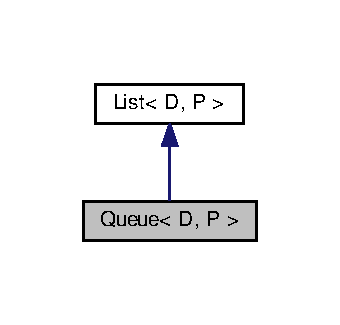
\includegraphics[width=163pt]{classQueue__inherit__graph}
\end{center}
\end{figure}


Collaboration diagram for Queue$<$ D, P $>$\+:
\nopagebreak
\begin{figure}[H]
\begin{center}
\leavevmode
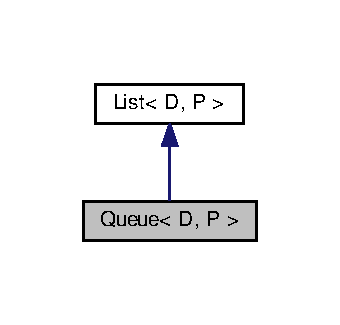
\includegraphics[width=163pt]{classQueue__coll__graph}
\end{center}
\end{figure}
\subsection*{Public Member Functions}
\begin{DoxyCompactItemize}
\item 
\hyperlink{classQueue_aaecc8eba91905e5bda9752e0f85a150e}{Queue} ()
\begin{DoxyCompactList}\small\item\em Constructor por defecto. Se crea con los atributos nulos y n en 0. \end{DoxyCompactList}\item 
virtual \hyperlink{classQueue_af88c0ebfc35932cdbbd75bae05e7a962}{$\sim$\+Queue} ()
\begin{DoxyCompactList}\small\item\em Destructor. L\+Lama al metodo empty\+List. \end{DoxyCompactList}\item 
void \hyperlink{classQueue_a63bd4d9779ddd75b2f78127337fe786a}{insert} (D data)
\begin{DoxyCompactList}\small\item\em Metodo para insertar un dato a una cola. Se crea una nueva celda y se enlaza a la ultima en caso de no haber ninguna se pone como la primera. \end{DoxyCompactList}\item 
void \hyperlink{classQueue_aa3d1a6edd30c4a9dda42e586db7f9fff}{remove} (D data)
\begin{DoxyCompactList}\small\item\em Metodo para remover una celda de la cola. \end{DoxyCompactList}\item 
P \& \hyperlink{classQueue_aefef2f172eaa0606944cdb4cf2fd5c53}{find} (D data)
\begin{DoxyCompactList}\small\item\em Metodo para encontrar un dato en la cola. \end{DoxyCompactList}\item 
D \& \hyperlink{classQueue_a1f2067f6e952bb0cec06087210b5ae2f}{get} (P \&cell)
\item 
int \hyperlink{classQueue_ab2c7217e6737bf579493b321184a2db3}{get\+Size} ()
\begin{DoxyCompactList}\small\item\em Metodo para encontrar el tamanno de la cola. \end{DoxyCompactList}\item 
void \hyperlink{classQueue_aa461f8fb363f960a6e0eb34b18503eaa}{print\+List} ()
\begin{DoxyCompactList}\small\item\em Metodo para imprimir la pila. \end{DoxyCompactList}\item 
P \& \hyperlink{classQueue_a989738789320704ae2d597e73919aefa}{next} (P \&cell)
\begin{DoxyCompactList}\small\item\em Metodo para encontrar la celda siguiente a una dada. \end{DoxyCompactList}\item 
P \& \hyperlink{classQueue_a238a908300566b4f9bb379216c7527c6}{prev} (P \&cell)
\begin{DoxyCompactList}\small\item\em Metodo para encontrar un puntero a la celda previa a una dada. \end{DoxyCompactList}\item 
void \hyperlink{classQueue_a37e23ca9e4ac29be510833bf6b7f6638}{empty\+List} ()
\begin{DoxyCompactList}\small\item\em Metodo para vaciar la pila. \end{DoxyCompactList}\item 
void \hyperlink{classQueue_aecdcae5571a7f0aebdf1c98f9ec382fa}{erase} (P $\ast$k)
\begin{DoxyCompactList}\small\item\em Metodo auxiliar para vaciar la pila. Trabaja recursivamente. \end{DoxyCompactList}\item 
void \hyperlink{classQueue_af8e5f753e54a7eb2a770c1bbf0c1d8fe}{assign} (P \&k, D d)
\item 
void \hyperlink{classQueue_a896b0e1bcac0d660079eb838c1823446}{sort} ()
\end{DoxyCompactItemize}
\subsection*{Data Fields}
\begin{DoxyCompactItemize}
\item 
P $\ast$ \hyperlink{classQueue_a1d8e79c486d52a6e8b329bf0f337fe06}{first}
\item 
P $\ast$ \hyperlink{classQueue_a466d5b8f1ec5d70fde748ac1b5c989c2}{last}
\end{DoxyCompactItemize}
\subsection*{Additional Inherited Members}


\subsection{Constructor \& Destructor Documentation}
\index{Queue@{Queue}!Queue@{Queue}}
\index{Queue@{Queue}!Queue@{Queue}}
\subsubsection[{\texorpdfstring{Queue()}{Queue()}}]{\setlength{\rightskip}{0pt plus 5cm}template$<$typename D , typename P $>$ {\bf Queue}$<$ D, P $>$\+::{\bf Queue} (
\begin{DoxyParamCaption}
{}
\end{DoxyParamCaption}
)\hspace{0.3cm}{\ttfamily [inline]}}\hypertarget{classQueue_aaecc8eba91905e5bda9752e0f85a150e}{}\label{classQueue_aaecc8eba91905e5bda9752e0f85a150e}


Constructor por defecto. Se crea con los atributos nulos y n en 0. 

\index{Queue@{Queue}!````~Queue@{$\sim$\+Queue}}
\index{````~Queue@{$\sim$\+Queue}!Queue@{Queue}}
\subsubsection[{\texorpdfstring{$\sim$\+Queue()}{~Queue()}}]{\setlength{\rightskip}{0pt plus 5cm}template$<$typename D , typename P $>$ virtual {\bf Queue}$<$ D, P $>$\+::$\sim${\bf Queue} (
\begin{DoxyParamCaption}
{}
\end{DoxyParamCaption}
)\hspace{0.3cm}{\ttfamily [inline]}, {\ttfamily [virtual]}}\hypertarget{classQueue_af88c0ebfc35932cdbbd75bae05e7a962}{}\label{classQueue_af88c0ebfc35932cdbbd75bae05e7a962}


Destructor. L\+Lama al metodo empty\+List. 



\subsection{Member Function Documentation}
\index{Queue@{Queue}!assign@{assign}}
\index{assign@{assign}!Queue@{Queue}}
\subsubsection[{\texorpdfstring{assign(\+P \&k, D d)}{assign(P &k, D d)}}]{\setlength{\rightskip}{0pt plus 5cm}template$<$typename D , typename P $>$ void {\bf Queue}$<$ D, P $>$\+::assign (
\begin{DoxyParamCaption}
\item[{P \&}]{k, }
\item[{D}]{d}
\end{DoxyParamCaption}
)\hspace{0.3cm}{\ttfamily [inline]}, {\ttfamily [virtual]}}\hypertarget{classQueue_af8e5f753e54a7eb2a770c1bbf0c1d8fe}{}\label{classQueue_af8e5f753e54a7eb2a770c1bbf0c1d8fe}


Implements \hyperlink{classList_a413440e7e102c944bec31ad5dce30b27}{List$<$ D, P $>$}.

\index{Queue@{Queue}!empty\+List@{empty\+List}}
\index{empty\+List@{empty\+List}!Queue@{Queue}}
\subsubsection[{\texorpdfstring{empty\+List()}{emptyList()}}]{\setlength{\rightskip}{0pt plus 5cm}template$<$typename D , typename P $>$ void {\bf Queue}$<$ D, P $>$\+::empty\+List (
\begin{DoxyParamCaption}
{}
\end{DoxyParamCaption}
)\hspace{0.3cm}{\ttfamily [inline]}, {\ttfamily [virtual]}}\hypertarget{classQueue_a37e23ca9e4ac29be510833bf6b7f6638}{}\label{classQueue_a37e23ca9e4ac29be510833bf6b7f6638}


Metodo para vaciar la pila. 



Implements \hyperlink{classList_a24b4f177a70215980e81ef7b2981fa1e}{List$<$ D, P $>$}.

\index{Queue@{Queue}!erase@{erase}}
\index{erase@{erase}!Queue@{Queue}}
\subsubsection[{\texorpdfstring{erase(\+P $\ast$k)}{erase(P *k)}}]{\setlength{\rightskip}{0pt plus 5cm}template$<$typename D , typename P $>$ void {\bf Queue}$<$ D, P $>$\+::erase (
\begin{DoxyParamCaption}
\item[{P $\ast$}]{k}
\end{DoxyParamCaption}
)\hspace{0.3cm}{\ttfamily [inline]}}\hypertarget{classQueue_aecdcae5571a7f0aebdf1c98f9ec382fa}{}\label{classQueue_aecdcae5571a7f0aebdf1c98f9ec382fa}


Metodo auxiliar para vaciar la pila. Trabaja recursivamente. 

\index{Queue@{Queue}!find@{find}}
\index{find@{find}!Queue@{Queue}}
\subsubsection[{\texorpdfstring{find(\+D data)}{find(D data)}}]{\setlength{\rightskip}{0pt plus 5cm}template$<$typename D , typename P $>$ P\& {\bf Queue}$<$ D, P $>$\+::find (
\begin{DoxyParamCaption}
\item[{D}]{data}
\end{DoxyParamCaption}
)\hspace{0.3cm}{\ttfamily [inline]}, {\ttfamily [virtual]}}\hypertarget{classQueue_aefef2f172eaa0606944cdb4cf2fd5c53}{}\label{classQueue_aefef2f172eaa0606944cdb4cf2fd5c53}


Metodo para encontrar un dato en la cola. 


\begin{DoxyParams}{Parameters}
{\em data} & Dato que queremos encontrar. \\
\hline
\end{DoxyParams}
\begin{DoxyReturn}{Returns}
Referencia de la cela que contiene dicho dato. 
\end{DoxyReturn}


Implements \hyperlink{classList_ae117dbe387f64f548fd0bddcc4d536dc}{List$<$ D, P $>$}.

\index{Queue@{Queue}!get@{get}}
\index{get@{get}!Queue@{Queue}}
\subsubsection[{\texorpdfstring{get(\+P \&cell)}{get(P &cell)}}]{\setlength{\rightskip}{0pt plus 5cm}template$<$typename D , typename P $>$ D\& {\bf Queue}$<$ D, P $>$\+::get (
\begin{DoxyParamCaption}
\item[{P \&}]{cell}
\end{DoxyParamCaption}
)\hspace{0.3cm}{\ttfamily [inline]}, {\ttfamily [virtual]}}\hypertarget{classQueue_a1f2067f6e952bb0cec06087210b5ae2f}{}\label{classQueue_a1f2067f6e952bb0cec06087210b5ae2f}


Implements \hyperlink{classList_afb5a777f30a186adce69028c387bf413}{List$<$ D, P $>$}.

\index{Queue@{Queue}!get\+Size@{get\+Size}}
\index{get\+Size@{get\+Size}!Queue@{Queue}}
\subsubsection[{\texorpdfstring{get\+Size()}{getSize()}}]{\setlength{\rightskip}{0pt plus 5cm}template$<$typename D , typename P $>$ int {\bf Queue}$<$ D, P $>$\+::get\+Size (
\begin{DoxyParamCaption}
{}
\end{DoxyParamCaption}
)\hspace{0.3cm}{\ttfamily [inline]}, {\ttfamily [virtual]}}\hypertarget{classQueue_ab2c7217e6737bf579493b321184a2db3}{}\label{classQueue_ab2c7217e6737bf579493b321184a2db3}


Metodo para encontrar el tamanno de la cola. 

\begin{DoxyReturn}{Returns}
Un entero con el numero de elementos que tiene la cola. 
\end{DoxyReturn}


Implements \hyperlink{classList_af213bbcf13ee436a0f04cde66e337672}{List$<$ D, P $>$}.

\index{Queue@{Queue}!insert@{insert}}
\index{insert@{insert}!Queue@{Queue}}
\subsubsection[{\texorpdfstring{insert(\+D data)}{insert(D data)}}]{\setlength{\rightskip}{0pt plus 5cm}template$<$typename D , typename P $>$ void {\bf Queue}$<$ D, P $>$\+::insert (
\begin{DoxyParamCaption}
\item[{D}]{data}
\end{DoxyParamCaption}
)\hspace{0.3cm}{\ttfamily [inline]}, {\ttfamily [virtual]}}\hypertarget{classQueue_a63bd4d9779ddd75b2f78127337fe786a}{}\label{classQueue_a63bd4d9779ddd75b2f78127337fe786a}


Metodo para insertar un dato a una cola. Se crea una nueva celda y se enlaza a la ultima en caso de no haber ninguna se pone como la primera. 


\begin{DoxyParams}{Parameters}
{\em data} & El dato que se quiere insertar. \\
\hline
{\em cell} & Celda que se crea para insertar el nuevo dato. \\
\hline
\end{DoxyParams}


Implements \hyperlink{classList_a01f588d87d47f8332928eca38f7b11bb}{List$<$ D, P $>$}.

\index{Queue@{Queue}!next@{next}}
\index{next@{next}!Queue@{Queue}}
\subsubsection[{\texorpdfstring{next(\+P \&cell)}{next(P &cell)}}]{\setlength{\rightskip}{0pt plus 5cm}template$<$typename D , typename P $>$ P\& {\bf Queue}$<$ D, P $>$\+::next (
\begin{DoxyParamCaption}
\item[{P \&}]{cell}
\end{DoxyParamCaption}
)\hspace{0.3cm}{\ttfamily [inline]}, {\ttfamily [virtual]}}\hypertarget{classQueue_a989738789320704ae2d597e73919aefa}{}\label{classQueue_a989738789320704ae2d597e73919aefa}


Metodo para encontrar la celda siguiente a una dada. 


\begin{DoxyParams}{Parameters}
{\em cell} & La celda de la cual que quiere la celda siguiente. \\
\hline
\end{DoxyParams}
\begin{DoxyReturn}{Returns}
Referencia de la celda siguiente a cell. 
\end{DoxyReturn}


Implements \hyperlink{classList_afa9ca2c678bc4f7d15ab0f4ab7c45421}{List$<$ D, P $>$}.

\index{Queue@{Queue}!prev@{prev}}
\index{prev@{prev}!Queue@{Queue}}
\subsubsection[{\texorpdfstring{prev(\+P \&cell)}{prev(P &cell)}}]{\setlength{\rightskip}{0pt plus 5cm}template$<$typename D , typename P $>$ P\& {\bf Queue}$<$ D, P $>$\+::prev (
\begin{DoxyParamCaption}
\item[{P \&}]{cell}
\end{DoxyParamCaption}
)\hspace{0.3cm}{\ttfamily [inline]}, {\ttfamily [virtual]}}\hypertarget{classQueue_a238a908300566b4f9bb379216c7527c6}{}\label{classQueue_a238a908300566b4f9bb379216c7527c6}


Metodo para encontrar un puntero a la celda previa a una dada. 


\begin{DoxyParams}{Parameters}
{\em cell} & La celda de la cual que quiere la celda previa. \\
\hline
\end{DoxyParams}
\begin{DoxyReturn}{Returns}
Puntero a la celda previa a cell. 
\end{DoxyReturn}


Implements \hyperlink{classList_a6c44364a04dff392b76e6a286074f3a1}{List$<$ D, P $>$}.

\index{Queue@{Queue}!print\+List@{print\+List}}
\index{print\+List@{print\+List}!Queue@{Queue}}
\subsubsection[{\texorpdfstring{print\+List()}{printList()}}]{\setlength{\rightskip}{0pt plus 5cm}template$<$typename D , typename P $>$ void {\bf Queue}$<$ D, P $>$\+::print\+List (
\begin{DoxyParamCaption}
{}
\end{DoxyParamCaption}
)\hspace{0.3cm}{\ttfamily [inline]}, {\ttfamily [virtual]}}\hypertarget{classQueue_aa461f8fb363f960a6e0eb34b18503eaa}{}\label{classQueue_aa461f8fb363f960a6e0eb34b18503eaa}


Metodo para imprimir la pila. 



Implements \hyperlink{classList_a8b34931e187e7e6b86aad86510ce4f3b}{List$<$ D, P $>$}.

\index{Queue@{Queue}!remove@{remove}}
\index{remove@{remove}!Queue@{Queue}}
\subsubsection[{\texorpdfstring{remove(\+D data)}{remove(D data)}}]{\setlength{\rightskip}{0pt plus 5cm}template$<$typename D , typename P $>$ void {\bf Queue}$<$ D, P $>$\+::remove (
\begin{DoxyParamCaption}
\item[{D}]{data}
\end{DoxyParamCaption}
)\hspace{0.3cm}{\ttfamily [inline]}, {\ttfamily [virtual]}}\hypertarget{classQueue_aa3d1a6edd30c4a9dda42e586db7f9fff}{}\label{classQueue_aa3d1a6edd30c4a9dda42e586db7f9fff}


Metodo para remover una celda de la cola. 


\begin{DoxyParams}{Parameters}
{\em data} & Este parametro no importa porque la cola solo puede eliminar una celda, la ultima. \\
\hline
\end{DoxyParams}


Implements \hyperlink{classList_a14fc4e853102018df78db3899aa00d71}{List$<$ D, P $>$}.

\index{Queue@{Queue}!sort@{sort}}
\index{sort@{sort}!Queue@{Queue}}
\subsubsection[{\texorpdfstring{sort()}{sort()}}]{\setlength{\rightskip}{0pt plus 5cm}template$<$typename D , typename P $>$ void {\bf Queue}$<$ D, P $>$\+::sort (
\begin{DoxyParamCaption}
{}
\end{DoxyParamCaption}
)\hspace{0.3cm}{\ttfamily [inline]}, {\ttfamily [virtual]}}\hypertarget{classQueue_a896b0e1bcac0d660079eb838c1823446}{}\label{classQueue_a896b0e1bcac0d660079eb838c1823446}


Implements \hyperlink{classList_ae3795939f27cf3e688cd470450e0c27a}{List$<$ D, P $>$}.



\subsection{Field Documentation}
\index{Queue@{Queue}!first@{first}}
\index{first@{first}!Queue@{Queue}}
\subsubsection[{\texorpdfstring{first}{first}}]{\setlength{\rightskip}{0pt plus 5cm}template$<$typename D , typename P $>$ P$\ast$ {\bf Queue}$<$ D, P $>$\+::first}\hypertarget{classQueue_a1d8e79c486d52a6e8b329bf0f337fe06}{}\label{classQueue_a1d8e79c486d52a6e8b329bf0f337fe06}
\index{Queue@{Queue}!last@{last}}
\index{last@{last}!Queue@{Queue}}
\subsubsection[{\texorpdfstring{last}{last}}]{\setlength{\rightskip}{0pt plus 5cm}template$<$typename D , typename P $>$ P$\ast$ {\bf Queue}$<$ D, P $>$\+::last}\hypertarget{classQueue_a466d5b8f1ec5d70fde748ac1b5c989c2}{}\label{classQueue_a466d5b8f1ec5d70fde748ac1b5c989c2}


The documentation for this class was generated from the following file\+:\begin{DoxyCompactItemize}
\item 
\hyperlink{Queue_8h}{Queue.\+h}\end{DoxyCompactItemize}

\hypertarget{classStack}{}\section{Stack$<$ D, P $>$ Class Template Reference}
\label{classStack}\index{Stack$<$ D, P $>$@{Stack$<$ D, P $>$}}


{\ttfamily \#include $<$Stack.\+h$>$}



Inheritance diagram for Stack$<$ D, P $>$\+:
\nopagebreak
\begin{figure}[H]
\begin{center}
\leavevmode
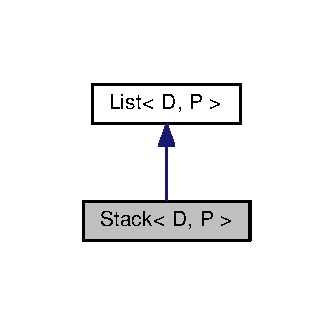
\includegraphics[width=160pt]{classStack__inherit__graph}
\end{center}
\end{figure}


Collaboration diagram for Stack$<$ D, P $>$\+:
\nopagebreak
\begin{figure}[H]
\begin{center}
\leavevmode
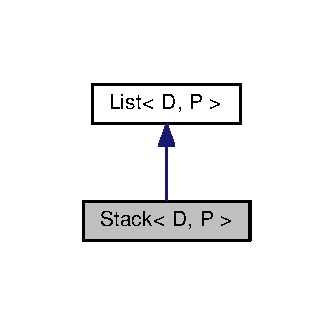
\includegraphics[width=160pt]{classStack__coll__graph}
\end{center}
\end{figure}
\subsection*{Public Member Functions}
\begin{DoxyCompactItemize}
\item 
\hyperlink{classStack_a6e0f84830cde41cb8d49818842d18d36}{Stack} ()
\begin{DoxyCompactList}\small\item\em Constructor por defecto. Se crea con los atributos nulos y n en 0. \end{DoxyCompactList}\item 
virtual \hyperlink{classStack_a063692d7f83addeb743eec7a3f97a957}{$\sim$\+Stack} ()
\begin{DoxyCompactList}\small\item\em Destructor. L\+Lama al metodo empty\+List. \end{DoxyCompactList}\item 
void \hyperlink{classStack_a2d8dfebafe6767cd668bcfc64d33bf63}{insert} (D data)
\begin{DoxyCompactList}\small\item\em Metodo para insertar un dato a una pila. Se crea una nueva celda y se enlaza a la ultima en caso de no haber ninguna se pone como la primera. \end{DoxyCompactList}\item 
void \hyperlink{classStack_a44889855bb26c4b1e050668959fab5be}{remove} (D data)
\begin{DoxyCompactList}\small\item\em Metodo para remover una celda de la pila. \end{DoxyCompactList}\item 
P \& \hyperlink{classStack_a2d24bac6bd65a0c90dd0dbe5c1297c1b}{find} (D data)
\begin{DoxyCompactList}\small\item\em Metodo para encontrar un dato en la pila. \end{DoxyCompactList}\item 
D \& \hyperlink{classStack_a488e4c5a68c70b5221df734fd953983f}{get} (P \&cell)
\item 
int \hyperlink{classStack_a74fc7e5921dfb247f9ad7052c3c4297a}{get\+Size} ()
\begin{DoxyCompactList}\small\item\em Metodo para encontrar el tamanno de la pila. \end{DoxyCompactList}\item 
void \hyperlink{classStack_a89b9967c15c83fe7c257a42e49725881}{print\+List} ()
\begin{DoxyCompactList}\small\item\em Metodo para imprimir la pila. \end{DoxyCompactList}\item 
P \& \hyperlink{classStack_aa86ccdcc6e57ade075de6ee51d1e5341}{next} (P \&cell)
\begin{DoxyCompactList}\small\item\em Metodo para encontrar la celda siguiente a una dada. \end{DoxyCompactList}\item 
P \& \hyperlink{classStack_a1e45de0c08c059313e99772c9e53820a}{prev} (P \&cell)
\item 
P $\ast$ \hyperlink{classStack_a0dfe15196e07fa8418a9f084db6b0173}{prevs} (P \&cell)
\begin{DoxyCompactList}\small\item\em Metodo para encontrar un puntero a la celda previa a una dada. \end{DoxyCompactList}\item 
void \hyperlink{classStack_a8d4119c8d4be2822f20a525743aa296e}{empty\+List} ()
\begin{DoxyCompactList}\small\item\em Metodo para vaciar la pila. \end{DoxyCompactList}\item 
void \hyperlink{classStack_ac2b9a59269d1ee3f593d42f81cf3a515}{erase} (P $\ast$k)
\begin{DoxyCompactList}\small\item\em Metodo auxiliar para vaciar la pila. Trabaja recursivamente. \end{DoxyCompactList}\item 
void \hyperlink{classStack_a8925b69439c6d583cf0a62f9a0cca026}{assign} (P \&k, D d)
\item 
void \hyperlink{classStack_a75261d2340f1f7b5e61b3770c0550982}{sort} ()
\end{DoxyCompactItemize}
\subsection*{Data Fields}
\begin{DoxyCompactItemize}
\item 
P $\ast$ \hyperlink{classStack_a072f08120143dbc8d868739fc24ae0b2}{first}
\item 
P $\ast$ \hyperlink{classStack_ac2caafb876777cbeb9306f9de407e00b}{last}
\end{DoxyCompactItemize}
\subsection*{Additional Inherited Members}


\subsection{Constructor \& Destructor Documentation}
\index{Stack@{Stack}!Stack@{Stack}}
\index{Stack@{Stack}!Stack@{Stack}}
\subsubsection[{\texorpdfstring{Stack()}{Stack()}}]{\setlength{\rightskip}{0pt plus 5cm}template$<$typename D , typename P $>$ {\bf Stack}$<$ D, P $>$\+::{\bf Stack} (
\begin{DoxyParamCaption}
{}
\end{DoxyParamCaption}
)\hspace{0.3cm}{\ttfamily [inline]}}\hypertarget{classStack_a6e0f84830cde41cb8d49818842d18d36}{}\label{classStack_a6e0f84830cde41cb8d49818842d18d36}


Constructor por defecto. Se crea con los atributos nulos y n en 0. 

\index{Stack@{Stack}!````~Stack@{$\sim$\+Stack}}
\index{````~Stack@{$\sim$\+Stack}!Stack@{Stack}}
\subsubsection[{\texorpdfstring{$\sim$\+Stack()}{~Stack()}}]{\setlength{\rightskip}{0pt plus 5cm}template$<$typename D , typename P $>$ virtual {\bf Stack}$<$ D, P $>$\+::$\sim${\bf Stack} (
\begin{DoxyParamCaption}
{}
\end{DoxyParamCaption}
)\hspace{0.3cm}{\ttfamily [inline]}, {\ttfamily [virtual]}}\hypertarget{classStack_a063692d7f83addeb743eec7a3f97a957}{}\label{classStack_a063692d7f83addeb743eec7a3f97a957}


Destructor. L\+Lama al metodo empty\+List. 



\subsection{Member Function Documentation}
\index{Stack@{Stack}!assign@{assign}}
\index{assign@{assign}!Stack@{Stack}}
\subsubsection[{\texorpdfstring{assign(\+P \&k, D d)}{assign(P &k, D d)}}]{\setlength{\rightskip}{0pt plus 5cm}template$<$typename D , typename P $>$ void {\bf Stack}$<$ D, P $>$\+::assign (
\begin{DoxyParamCaption}
\item[{P \&}]{k, }
\item[{D}]{d}
\end{DoxyParamCaption}
)\hspace{0.3cm}{\ttfamily [inline]}, {\ttfamily [virtual]}}\hypertarget{classStack_a8925b69439c6d583cf0a62f9a0cca026}{}\label{classStack_a8925b69439c6d583cf0a62f9a0cca026}


Implements \hyperlink{classList_a413440e7e102c944bec31ad5dce30b27}{List$<$ D, P $>$}.

\index{Stack@{Stack}!empty\+List@{empty\+List}}
\index{empty\+List@{empty\+List}!Stack@{Stack}}
\subsubsection[{\texorpdfstring{empty\+List()}{emptyList()}}]{\setlength{\rightskip}{0pt plus 5cm}template$<$typename D , typename P $>$ void {\bf Stack}$<$ D, P $>$\+::empty\+List (
\begin{DoxyParamCaption}
{}
\end{DoxyParamCaption}
)\hspace{0.3cm}{\ttfamily [inline]}, {\ttfamily [virtual]}}\hypertarget{classStack_a8d4119c8d4be2822f20a525743aa296e}{}\label{classStack_a8d4119c8d4be2822f20a525743aa296e}


Metodo para vaciar la pila. 



Implements \hyperlink{classList_a24b4f177a70215980e81ef7b2981fa1e}{List$<$ D, P $>$}.

\index{Stack@{Stack}!erase@{erase}}
\index{erase@{erase}!Stack@{Stack}}
\subsubsection[{\texorpdfstring{erase(\+P $\ast$k)}{erase(P *k)}}]{\setlength{\rightskip}{0pt plus 5cm}template$<$typename D , typename P $>$ void {\bf Stack}$<$ D, P $>$\+::erase (
\begin{DoxyParamCaption}
\item[{P $\ast$}]{k}
\end{DoxyParamCaption}
)\hspace{0.3cm}{\ttfamily [inline]}}\hypertarget{classStack_ac2b9a59269d1ee3f593d42f81cf3a515}{}\label{classStack_ac2b9a59269d1ee3f593d42f81cf3a515}


Metodo auxiliar para vaciar la pila. Trabaja recursivamente. 

\index{Stack@{Stack}!find@{find}}
\index{find@{find}!Stack@{Stack}}
\subsubsection[{\texorpdfstring{find(\+D data)}{find(D data)}}]{\setlength{\rightskip}{0pt plus 5cm}template$<$typename D , typename P $>$ P\& {\bf Stack}$<$ D, P $>$\+::find (
\begin{DoxyParamCaption}
\item[{D}]{data}
\end{DoxyParamCaption}
)\hspace{0.3cm}{\ttfamily [inline]}, {\ttfamily [virtual]}}\hypertarget{classStack_a2d24bac6bd65a0c90dd0dbe5c1297c1b}{}\label{classStack_a2d24bac6bd65a0c90dd0dbe5c1297c1b}


Metodo para encontrar un dato en la pila. 


\begin{DoxyParams}{Parameters}
{\em data} & Dato que queremos encontrar. \\
\hline
\end{DoxyParams}
\begin{DoxyReturn}{Returns}
Referencia de la cela que contiene dicho dato. 
\end{DoxyReturn}


Implements \hyperlink{classList_ae117dbe387f64f548fd0bddcc4d536dc}{List$<$ D, P $>$}.

\index{Stack@{Stack}!get@{get}}
\index{get@{get}!Stack@{Stack}}
\subsubsection[{\texorpdfstring{get(\+P \&cell)}{get(P &cell)}}]{\setlength{\rightskip}{0pt plus 5cm}template$<$typename D , typename P $>$ D\& {\bf Stack}$<$ D, P $>$\+::get (
\begin{DoxyParamCaption}
\item[{P \&}]{cell}
\end{DoxyParamCaption}
)\hspace{0.3cm}{\ttfamily [inline]}, {\ttfamily [virtual]}}\hypertarget{classStack_a488e4c5a68c70b5221df734fd953983f}{}\label{classStack_a488e4c5a68c70b5221df734fd953983f}


Implements \hyperlink{classList_afb5a777f30a186adce69028c387bf413}{List$<$ D, P $>$}.

\index{Stack@{Stack}!get\+Size@{get\+Size}}
\index{get\+Size@{get\+Size}!Stack@{Stack}}
\subsubsection[{\texorpdfstring{get\+Size()}{getSize()}}]{\setlength{\rightskip}{0pt plus 5cm}template$<$typename D , typename P $>$ int {\bf Stack}$<$ D, P $>$\+::get\+Size (
\begin{DoxyParamCaption}
{}
\end{DoxyParamCaption}
)\hspace{0.3cm}{\ttfamily [inline]}, {\ttfamily [virtual]}}\hypertarget{classStack_a74fc7e5921dfb247f9ad7052c3c4297a}{}\label{classStack_a74fc7e5921dfb247f9ad7052c3c4297a}


Metodo para encontrar el tamanno de la pila. 

\begin{DoxyReturn}{Returns}
Un entero con el numero de elementos que tiene la pila. 
\end{DoxyReturn}


Implements \hyperlink{classList_af213bbcf13ee436a0f04cde66e337672}{List$<$ D, P $>$}.

\index{Stack@{Stack}!insert@{insert}}
\index{insert@{insert}!Stack@{Stack}}
\subsubsection[{\texorpdfstring{insert(\+D data)}{insert(D data)}}]{\setlength{\rightskip}{0pt plus 5cm}template$<$typename D , typename P $>$ void {\bf Stack}$<$ D, P $>$\+::insert (
\begin{DoxyParamCaption}
\item[{D}]{data}
\end{DoxyParamCaption}
)\hspace{0.3cm}{\ttfamily [inline]}, {\ttfamily [virtual]}}\hypertarget{classStack_a2d8dfebafe6767cd668bcfc64d33bf63}{}\label{classStack_a2d8dfebafe6767cd668bcfc64d33bf63}


Metodo para insertar un dato a una pila. Se crea una nueva celda y se enlaza a la ultima en caso de no haber ninguna se pone como la primera. 


\begin{DoxyParams}{Parameters}
{\em data} & El dato que se quiere insertar. \\
\hline
{\em cell} & Celda que se crea para insertar el nuevo dato. \\
\hline
\end{DoxyParams}


Implements \hyperlink{classList_a01f588d87d47f8332928eca38f7b11bb}{List$<$ D, P $>$}.

\index{Stack@{Stack}!next@{next}}
\index{next@{next}!Stack@{Stack}}
\subsubsection[{\texorpdfstring{next(\+P \&cell)}{next(P &cell)}}]{\setlength{\rightskip}{0pt plus 5cm}template$<$typename D , typename P $>$ P\& {\bf Stack}$<$ D, P $>$\+::next (
\begin{DoxyParamCaption}
\item[{P \&}]{cell}
\end{DoxyParamCaption}
)\hspace{0.3cm}{\ttfamily [inline]}, {\ttfamily [virtual]}}\hypertarget{classStack_aa86ccdcc6e57ade075de6ee51d1e5341}{}\label{classStack_aa86ccdcc6e57ade075de6ee51d1e5341}


Metodo para encontrar la celda siguiente a una dada. 


\begin{DoxyParams}{Parameters}
{\em cell} & La celda de la cual que quiere la celda siguiente. \\
\hline
\end{DoxyParams}
\begin{DoxyReturn}{Returns}
Referencia de la celda siguiente a cell. 
\end{DoxyReturn}


Implements \hyperlink{classList_afa9ca2c678bc4f7d15ab0f4ab7c45421}{List$<$ D, P $>$}.

\index{Stack@{Stack}!prev@{prev}}
\index{prev@{prev}!Stack@{Stack}}
\subsubsection[{\texorpdfstring{prev(\+P \&cell)}{prev(P &cell)}}]{\setlength{\rightskip}{0pt plus 5cm}template$<$typename D , typename P $>$ P\& {\bf Stack}$<$ D, P $>$\+::prev (
\begin{DoxyParamCaption}
\item[{P \&}]{cell}
\end{DoxyParamCaption}
)\hspace{0.3cm}{\ttfamily [inline]}, {\ttfamily [virtual]}}\hypertarget{classStack_a1e45de0c08c059313e99772c9e53820a}{}\label{classStack_a1e45de0c08c059313e99772c9e53820a}


Implements \hyperlink{classList_a6c44364a04dff392b76e6a286074f3a1}{List$<$ D, P $>$}.

\index{Stack@{Stack}!prevs@{prevs}}
\index{prevs@{prevs}!Stack@{Stack}}
\subsubsection[{\texorpdfstring{prevs(\+P \&cell)}{prevs(P &cell)}}]{\setlength{\rightskip}{0pt plus 5cm}template$<$typename D , typename P $>$ P$\ast$ {\bf Stack}$<$ D, P $>$\+::prevs (
\begin{DoxyParamCaption}
\item[{P \&}]{cell}
\end{DoxyParamCaption}
)\hspace{0.3cm}{\ttfamily [inline]}}\hypertarget{classStack_a0dfe15196e07fa8418a9f084db6b0173}{}\label{classStack_a0dfe15196e07fa8418a9f084db6b0173}


Metodo para encontrar un puntero a la celda previa a una dada. 


\begin{DoxyParams}{Parameters}
{\em cell} & La celda de la cual que quiere la celda previa. \\
\hline
\end{DoxyParams}
\begin{DoxyReturn}{Returns}
Puntero a la celda previa a cell. 
\end{DoxyReturn}
\index{Stack@{Stack}!print\+List@{print\+List}}
\index{print\+List@{print\+List}!Stack@{Stack}}
\subsubsection[{\texorpdfstring{print\+List()}{printList()}}]{\setlength{\rightskip}{0pt plus 5cm}template$<$typename D , typename P $>$ void {\bf Stack}$<$ D, P $>$\+::print\+List (
\begin{DoxyParamCaption}
{}
\end{DoxyParamCaption}
)\hspace{0.3cm}{\ttfamily [inline]}, {\ttfamily [virtual]}}\hypertarget{classStack_a89b9967c15c83fe7c257a42e49725881}{}\label{classStack_a89b9967c15c83fe7c257a42e49725881}


Metodo para imprimir la pila. 



Implements \hyperlink{classList_a8b34931e187e7e6b86aad86510ce4f3b}{List$<$ D, P $>$}.

\index{Stack@{Stack}!remove@{remove}}
\index{remove@{remove}!Stack@{Stack}}
\subsubsection[{\texorpdfstring{remove(\+D data)}{remove(D data)}}]{\setlength{\rightskip}{0pt plus 5cm}template$<$typename D , typename P $>$ void {\bf Stack}$<$ D, P $>$\+::remove (
\begin{DoxyParamCaption}
\item[{D}]{data}
\end{DoxyParamCaption}
)\hspace{0.3cm}{\ttfamily [inline]}, {\ttfamily [virtual]}}\hypertarget{classStack_a44889855bb26c4b1e050668959fab5be}{}\label{classStack_a44889855bb26c4b1e050668959fab5be}


Metodo para remover una celda de la pila. 


\begin{DoxyParams}{Parameters}
{\em data} & Este parametro no importa porque la pila solo puede eliminar una celda, la ultima. \\
\hline
\end{DoxyParams}


Implements \hyperlink{classList_a14fc4e853102018df78db3899aa00d71}{List$<$ D, P $>$}.

\index{Stack@{Stack}!sort@{sort}}
\index{sort@{sort}!Stack@{Stack}}
\subsubsection[{\texorpdfstring{sort()}{sort()}}]{\setlength{\rightskip}{0pt plus 5cm}template$<$typename D , typename P $>$ void {\bf Stack}$<$ D, P $>$\+::sort (
\begin{DoxyParamCaption}
{}
\end{DoxyParamCaption}
)\hspace{0.3cm}{\ttfamily [inline]}, {\ttfamily [virtual]}}\hypertarget{classStack_a75261d2340f1f7b5e61b3770c0550982}{}\label{classStack_a75261d2340f1f7b5e61b3770c0550982}


Implements \hyperlink{classList_ae3795939f27cf3e688cd470450e0c27a}{List$<$ D, P $>$}.



\subsection{Field Documentation}
\index{Stack@{Stack}!first@{first}}
\index{first@{first}!Stack@{Stack}}
\subsubsection[{\texorpdfstring{first}{first}}]{\setlength{\rightskip}{0pt plus 5cm}template$<$typename D , typename P $>$ P$\ast$ {\bf Stack}$<$ D, P $>$\+::first}\hypertarget{classStack_a072f08120143dbc8d868739fc24ae0b2}{}\label{classStack_a072f08120143dbc8d868739fc24ae0b2}
\index{Stack@{Stack}!last@{last}}
\index{last@{last}!Stack@{Stack}}
\subsubsection[{\texorpdfstring{last}{last}}]{\setlength{\rightskip}{0pt plus 5cm}template$<$typename D , typename P $>$ P$\ast$ {\bf Stack}$<$ D, P $>$\+::last}\hypertarget{classStack_ac2caafb876777cbeb9306f9de407e00b}{}\label{classStack_ac2caafb876777cbeb9306f9de407e00b}


The documentation for this class was generated from the following file\+:\begin{DoxyCompactItemize}
\item 
\hyperlink{Stack_8h}{Stack.\+h}\end{DoxyCompactItemize}

\chapter{File Documentation}
\hypertarget{Cell_8h}{}\section{Cell.\+h File Reference}
\label{Cell_8h}\index{Cell.\+h@{Cell.\+h}}
This graph shows which files directly or indirectly include this file\+:
\nopagebreak
\begin{figure}[H]
\begin{center}
\leavevmode
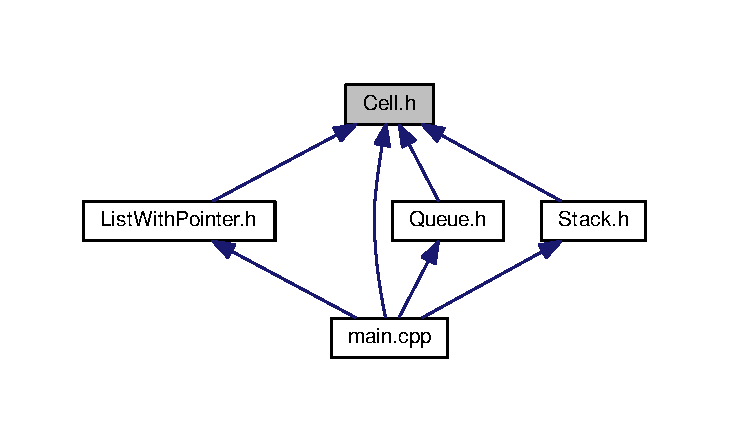
\includegraphics[width=183pt]{Cell_8h__dep__incl}
\end{center}
\end{figure}
\subsection*{Data Structures}
\begin{DoxyCompactItemize}
\item 
class \hyperlink{classCell}{Cell$<$ D $>$}
\end{DoxyCompactItemize}

\hypertarget{List_8h}{}\section{List.\+h File Reference}
\label{List_8h}\index{List.\+h@{List.\+h}}
This graph shows which files directly or indirectly include this file\+:
\nopagebreak
\begin{figure}[H]
\begin{center}
\leavevmode
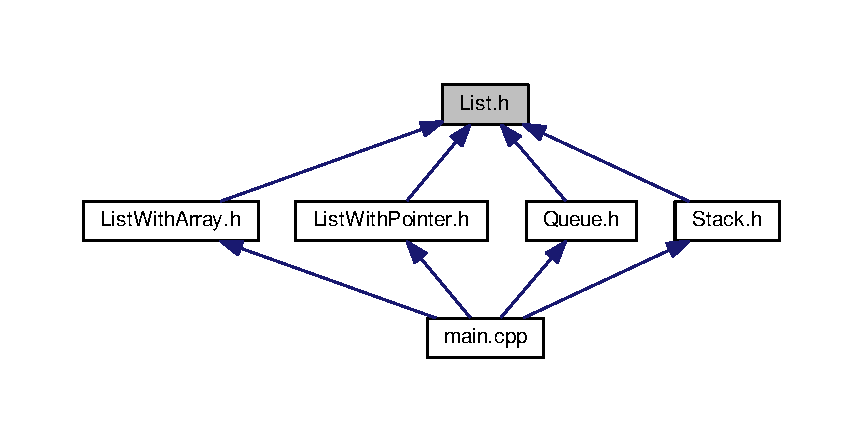
\includegraphics[width=183pt]{List_8h__dep__incl}
\end{center}
\end{figure}
\subsection*{Data Structures}
\begin{DoxyCompactItemize}
\item 
class \hyperlink{classList}{List$<$ D, P $>$}
\end{DoxyCompactItemize}

\hypertarget{ListWithArray_8h}{}\section{List\+With\+Array.\+h File Reference}
\label{ListWithArray_8h}\index{List\+With\+Array.\+h@{List\+With\+Array.\+h}}
{\ttfamily \#include $<$iostream$>$}\\*
{\ttfamily \#include \char`\"{}List.\+h\char`\"{}}\\*
{\ttfamily \#include \char`\"{}My\+Int.\+h\char`\"{}}\\*
Include dependency graph for List\+With\+Array.\+h\+:
\nopagebreak
\begin{figure}[H]
\begin{center}
\leavevmode
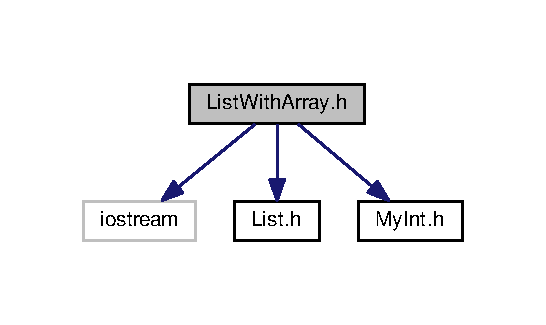
\includegraphics[width=262pt]{ListWithArray_8h__incl}
\end{center}
\end{figure}
This graph shows which files directly or indirectly include this file\+:
\nopagebreak
\begin{figure}[H]
\begin{center}
\leavevmode
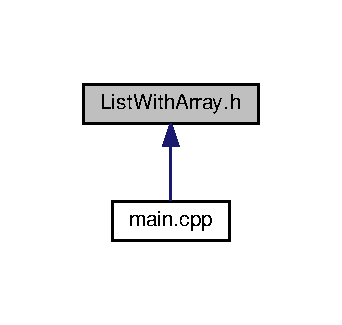
\includegraphics[width=164pt]{ListWithArray_8h__dep__incl}
\end{center}
\end{figure}
\subsection*{Data Structures}
\begin{DoxyCompactItemize}
\item 
class \hyperlink{classListWithArray}{List\+With\+Array$<$ D, P $>$}
\end{DoxyCompactItemize}

\hypertarget{ListWithPointer_8h}{}\section{List\+With\+Pointer.\+h File Reference}
\label{ListWithPointer_8h}\index{List\+With\+Pointer.\+h@{List\+With\+Pointer.\+h}}
{\ttfamily \#include $<$iostream$>$}\\*
{\ttfamily \#include \char`\"{}Cell.\+h\char`\"{}}\\*
{\ttfamily \#include \char`\"{}List.\+h\char`\"{}}\\*
Include dependency graph for List\+With\+Pointer.\+h\+:
\nopagebreak
\begin{figure}[H]
\begin{center}
\leavevmode
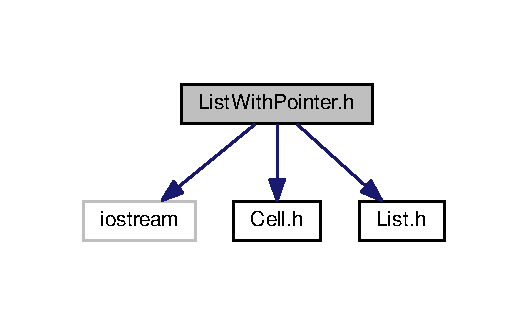
\includegraphics[width=254pt]{ListWithPointer_8h__incl}
\end{center}
\end{figure}
This graph shows which files directly or indirectly include this file\+:
\nopagebreak
\begin{figure}[H]
\begin{center}
\leavevmode
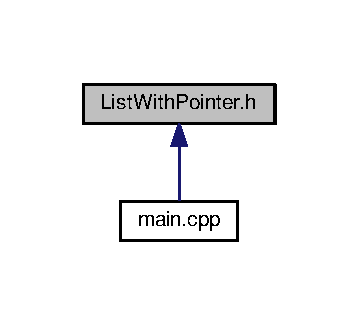
\includegraphics[width=172pt]{ListWithPointer_8h__dep__incl}
\end{center}
\end{figure}
\subsection*{Data Structures}
\begin{DoxyCompactItemize}
\item 
class \hyperlink{classListWithPointer}{List\+With\+Pointer$<$ D, P $>$}
\end{DoxyCompactItemize}

\hypertarget{main_8cpp}{}\section{main.\+cpp File Reference}
\label{main_8cpp}\index{main.\+cpp@{main.\+cpp}}
{\ttfamily \#include $<$stdlib.\+h$>$}\\*
{\ttfamily \#include \char`\"{}Controlador.\+h\char`\"{}}\\*
Include dependency graph for main.\+cpp\+:\nopagebreak
\begin{figure}[H]
\begin{center}
\leavevmode
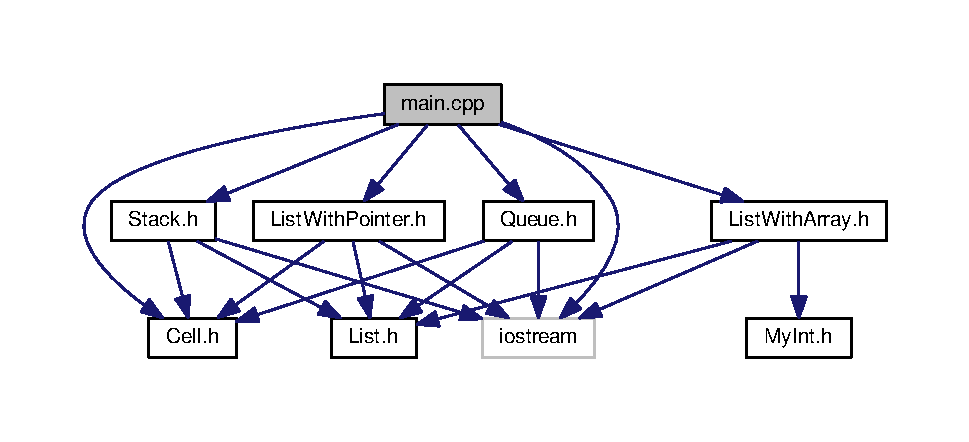
\includegraphics[width=350pt]{main_8cpp__incl}
\end{center}
\end{figure}
\subsection*{Functions}
\begin{DoxyCompactItemize}
\item 
int \hyperlink{main_8cpp_a0ddf1224851353fc92bfbff6f499fa97}{main} (int argc, char $\ast$argv\mbox{[}$\,$\mbox{]})
\end{DoxyCompactItemize}


\subsection{Function Documentation}
\index{main.\+cpp@{main.\+cpp}!main@{main}}
\index{main@{main}!main.\+cpp@{main.\+cpp}}
\subsubsection[{\texorpdfstring{main(int argc, char $\ast$argv[])}{main(int argc, char *argv[])}}]{\setlength{\rightskip}{0pt plus 5cm}int main (
\begin{DoxyParamCaption}
\item[{int}]{argc, }
\item[{char $\ast$}]{argv\mbox{[}$\,$\mbox{]}}
\end{DoxyParamCaption}
)}\hypertarget{main_8cpp_a0ddf1224851353fc92bfbff6f499fa97}{}\label{main_8cpp_a0ddf1224851353fc92bfbff6f499fa97}

\hypertarget{MyInt_8h}{}\section{My\+Int.\+h File Reference}
\label{MyInt_8h}\index{My\+Int.\+h@{My\+Int.\+h}}
This graph shows which files directly or indirectly include this file\+:
\nopagebreak
\begin{figure}[H]
\begin{center}
\leavevmode
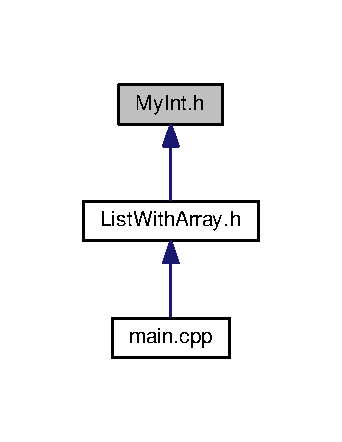
\includegraphics[width=164pt]{MyInt_8h__dep__incl}
\end{center}
\end{figure}
\subsection*{Data Structures}
\begin{DoxyCompactItemize}
\item 
class \hyperlink{classMyInt}{My\+Int}
\end{DoxyCompactItemize}

\hypertarget{Queue_8h}{}\section{Queue.\+h File Reference}
\label{Queue_8h}\index{Queue.\+h@{Queue.\+h}}
{\ttfamily \#include $<$iostream$>$}\\*
{\ttfamily \#include \char`\"{}Cell.\+h\char`\"{}}\\*
{\ttfamily \#include \char`\"{}List.\+h\char`\"{}}\\*
Include dependency graph for Queue.\+h\+:
\nopagebreak
\begin{figure}[H]
\begin{center}
\leavevmode
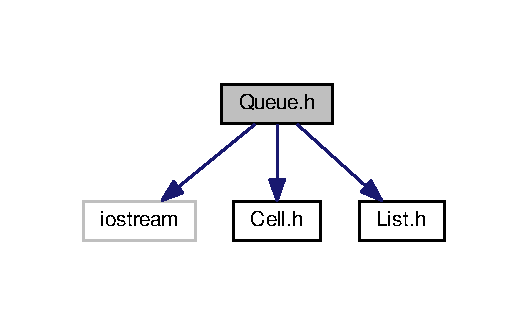
\includegraphics[width=254pt]{Queue_8h__incl}
\end{center}
\end{figure}
This graph shows which files directly or indirectly include this file\+:
\nopagebreak
\begin{figure}[H]
\begin{center}
\leavevmode
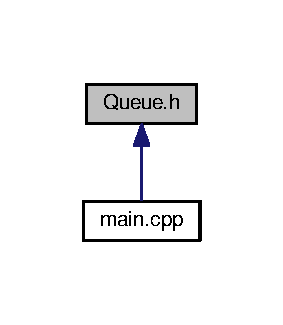
\includegraphics[width=136pt]{Queue_8h__dep__incl}
\end{center}
\end{figure}
\subsection*{Data Structures}
\begin{DoxyCompactItemize}
\item 
class \hyperlink{classQueue}{Queue$<$ D, P $>$}
\end{DoxyCompactItemize}

\hypertarget{Stack_8h}{}\section{Stack.\+h File Reference}
\label{Stack_8h}\index{Stack.\+h@{Stack.\+h}}
{\ttfamily \#include $<$iostream$>$}\\*
{\ttfamily \#include \char`\"{}Cell.\+h\char`\"{}}\\*
{\ttfamily \#include \char`\"{}List.\+h\char`\"{}}\\*
Include dependency graph for Stack.\+h\+:
\nopagebreak
\begin{figure}[H]
\begin{center}
\leavevmode
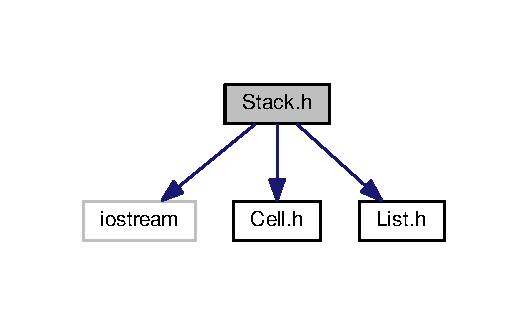
\includegraphics[width=254pt]{Stack_8h__incl}
\end{center}
\end{figure}
This graph shows which files directly or indirectly include this file\+:
\nopagebreak
\begin{figure}[H]
\begin{center}
\leavevmode
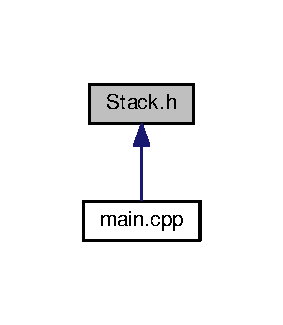
\includegraphics[width=136pt]{Stack_8h__dep__incl}
\end{center}
\end{figure}
\subsection*{Data Structures}
\begin{DoxyCompactItemize}
\item 
class \hyperlink{classStack}{Stack$<$ D, P $>$}
\end{DoxyCompactItemize}

%--- End generated contents ---

% Index
\backmatter
\newpage
\phantomsection
\clearemptydoublepage
\addcontentsline{toc}{chapter}{Index}
\printindex

\end{document}
